%%
%% Automatically generated file from DocOnce source
%% (https://github.com/hplgit/doconce/)
%%


%-------------------- begin preamble ----------------------

\documentclass[%
twoside,                 % oneside: electronic viewing, twoside: printing
final,                   % or draft (marks overfull hboxes, figures with paths)
chapterprefix=true,      % "Chapter" word at beginning of each chapter
open=right               % start new chapters on odd-numbered pages
10pt]{book}

\listfiles               % print all files needed to compile this document

\usepackage{relsize,epsfig,makeidx,color,setspace,amsmath,amsfonts}
\usepackage[table]{xcolor}
\usepackage{bm,microtype}

\usepackage{fancyvrb} % packages needed for verbatim environments


\usepackage[T1]{fontenc}
%\usepackage[latin1]{inputenc}
\usepackage[utf8]{inputenc}

\usepackage{lmodern}         % Latin Modern fonts derived from Computer Modern

% Hyperlinks in PDF:
\definecolor{linkcolor}{rgb}{0,0,0.4}
\usepackage[%
    colorlinks=true,
    linkcolor=linkcolor,
    urlcolor=linkcolor,
    citecolor=black,
    filecolor=black,
    %filecolor=blue,
    pdfmenubar=true,
    pdftoolbar=true,
    bookmarksdepth=3   % Uncomment (and tweak) for PDF bookmarks with more levels than the TOC
            ]{hyperref}
%\hyperbaseurl{}   % hyperlinks are relative to this root

\setcounter{tocdepth}{2}  % number chapter, section, subsection

% Tricks for having figures close to where they are defined:
% 1. define less restrictive rules for where to put figures
\setcounter{topnumber}{2}
\setcounter{bottomnumber}{2}
\setcounter{totalnumber}{4}
\renewcommand{\topfraction}{0.85}
\renewcommand{\bottomfraction}{0.85}
\renewcommand{\textfraction}{0.15}
\renewcommand{\floatpagefraction}{0.7}
% 2. ensure all figures are flushed before next section
\usepackage[section]{placeins}
% 3. enable begin{figure}[H] (often leads to ugly pagebreaks)
%\usepackage{float}\restylefloat{figure}

% prevent orhpans and widows
\clubpenalty = 10000
\widowpenalty = 10000

% Make sure blank even-numbered pages before new chapters are
% totally blank with no header
\newcommand{\clearemptydoublepage}{\clearpage{\pagestyle{empty}\cleardoublepage}}
%\let\cleardoublepage\clearemptydoublepage % caused error in the toc

% --- end of standard preamble for documents ---


% insert custom LaTeX commands...

\raggedbottom
\makeindex

%-------------------- end preamble ----------------------

\begin{document}



% ------------------- main content ----------------------



% ----------------- title -------------------------

\thispagestyle{empty}

\begin{center}
{\LARGE\bf
\begin{spacing}{1.25}
Geographic models 
\end{spacing}
}
\end{center}

% ----------------- author(s) -------------------------

\begin{center}
{\bf Torbjørn Seland${}^{}$} \\ [0mm]
\end{center}

    \begin{center}
% List of all institutions:
\end{center}

% ----------------- end author(s) -------------------------

\begin{center}
Dec 18, 2014
\end{center}

\vspace{1cm}


\tableofcontents


\vspace{1cm} % after toc




\newcommand{\Imax}{I_{\textrm{max}}}

\chapter{PDE models}
This chapter will introduce a spatial model for epidemic diseases. The ODE system from the previously chapter~\ref{section:ODE_models} can be expanded with a term for geographic spread of the disease. The first section \emph{Simple system for spatial spread} will be based on the simple SIR model presented in previously chapter, and the chapter \emph{Geographic spread and Control of epidemics} by Murray \cite{murray2003mathematical}. The parameters from the \emph{English Boarding School} in the previously chapter will be used for the model and the results will be compared. The position of the infected student will be studied to see if it affects the number in the \emph{Infected} group. The last section, \emph{Zombiefication}, will study and expand the system from Langtangen, Mardal and Røtnes \cite{zombie-math}. The results and parameter values used to calculate \emph{Walking Dead} will be compared with the previously ODE system and variations of this PDE. 


\section{Simple system for spatial spread}
A spatial variable, \textbf{x}, will be introduced to the model. This results in both temporal and spatial variations. The difference from a standard ODE system will be the diffusion part added to each equation. The system can be seen in Eq.(\ref{eq:simple_PDE}). 
\begin{equation} \label{eq:simple_PDE}
	\begin{aligned}
	\frac{\partial S}{\partial t} &= -rIS + D\nabla ^2 S\\
	\frac{\partial I}{\partial t} &= rIS- aI + D\nabla ^2 I\\
	\frac{\partial R}{\partial t} &= aI + D\nabla ^2 R
	\end{aligned}
\end{equation}
Here $S$ describes the \emph{Susceptible} group, $I$ describes the \emph{Infected} group and $R$ describes the \emph{Removed} group. The following conditions are set for the boundary and initial values:
\begin{equation} \label{eq:boundary_initial}
	\begin{aligned}
	u_x(0,t) &= u_x(X,t) = 0,\quad u = S,I,R\\
	u(x,0) &= f_u(x),\quad u= S,I,R
	\end{aligned}
\end{equation}
This results in Neumann conditions at the boundary. The following implementation can be used at the boundary
\begin{equation}
	\begin{aligned}
	\frac{u_{-1}^n - u_1^n}{2\Delta x} &= 0 \\
	u_{-1}^n &= u_1^n
	\end{aligned}
\end{equation}
This is solved by adding an extra point on each side, called ghost points. The values in these ghost points are updated every time step with values from $u_1^n$ and $u_{X-1}^n$. All three groups, $S,I,R$ in Eq.(\ref{eq:simple_PDE}) have the same diffusion coefficient, $D$. This gives the three groups the same diffusion speed. This can vary between systems. Later in the chapter, in section \emph{Zombiefication}, different diffusion terms are given to the groups. The two probabilities $rIS$ and $aI$ will work in the same way as in the ODE system. Since this model takes the position into account, a group of \emph{Infected} that move into a uniform population with \emph{Susceptible} can be model. The group of \emph{Susceptible} has the density $S_0$. A simulation can show the geotemporal spread of the disease. The problem can first be considered as one-dimensional. The system can be nondimensionalised by writing 
\begin{equation} \label{eq:constants_nondimensional}
	\begin{aligned}
	I^* =\frac{I}{S_0},&\quad I^* = \frac{I}{S_0},&\quad R^*= \frac{R}{S_0},&\\
	x^* =\left(\frac{rS_0}{D}\right)^{1/2}x,&\quad t^*=rS_0t,&\quad \lambda =\frac{a}{rS_0},&
	\end{aligned}
\end{equation}
$S_0$ is used as a representative population. Now Eq.(\ref{eq:simple_PDE}) can be expressed as in Eq.(\ref{eq:simple_non_PDE}). The asterisks have been dropped to make it easier to read.
\begin{equation} \label{eq:simple_non_PDE}
	\begin{aligned}
	\frac{\partial S}{\partial t} &= -IS + \frac{\partial^2 S}{\partial x^2},\\
	\frac{\partial I}{\partial t} &= IS- \lambda I + \frac{\partial^2 I}{\partial x^2},\\
	\frac{\partial R}{\partial t} &= \lambda I + \frac{\partial^2 R}{\partial x^2},
	\end{aligned}
\end{equation}
The three parameters $r$, $a$ and $D$ have been replaced by $\lambda$. The \emph{reproduction rate} that was presented for the ODE model can be seen as $1/\lambda $.
\begin{equation} \label{eq:reproduction_rate_PDF}
R_0 = \frac{1}{\lambda} = \frac{rS_0}{a}
\end{equation}
The number of secondary infections produced by one primary infected can be seen as $1/\lambda$. It can also be used to measure two different time scales. The first one, $1/(rS_0)$, measures the contagious time of the disease. The second one looks at the life expectancy for an infected. This can be described as $1/a$ \cite{murray2003mathematical}. 
\subsection{Travelling wave 1D}
In this case the travelling wave describes how a group of \emph{Infected} travels through a geographic area of \emph{Susceptible}. This will be shown by sending a pulse from the \emph{Infected} group into a group of \emph{Susceptible}. A travelling wave solution can be described as follows,
\begin{equation} \label{eq:trav_para}
I(x,t)=I(z),\quad S(x,t)=S(z),\quad R(x,t) = R(z),\quad z = x-ct,
\end{equation}
The value $c$ describes the wave speed. This represents a wave of constant shape that travels in the positive x-direction. Eq.(\ref{eq:trav_para}) can be inserted into Eq.(\ref{eq:simple_non_PDE}). This result in the ordinary system Eq.(\ref{eq:ord_diff_sys})
\begin{equation} \label{eq:ord_diff_sys}
	\begin{aligned}
	S'' + cS' - IS &= 0,\\
	I'' + cI' + I(S-\lambda)&=0\\
	R'' + cR  + I\lambda &=0
	\end{aligned}
\end{equation}
This makes an eigenvalue problem. The value of $\lambda$ needs to stay in a range where $c > 0$ is fulfilled. The values $S$, $I$ and $R$ have to stay nonnegative. This leads to
\begin{equation} 
	\begin{aligned}
	0 \leq S(-\infty) < S(\infty)&=1\\
	I(-\infty)=I(\infty)&=0,\\
	1 \geq R(-\infty)\geq R(\infty) &= 0
	\end{aligned}
\end{equation}
An epidemic wave can be seen in Fig.(\ref{fig:1D_sub}). The value of $\lambda$ is set to 0.5. The initial value of \emph{Susceptible} is 1 for the area and the \emph{Removed} is set to 0. The \emph{Infected} group has a Gauss curve around 0 at initial time. In the four subplots in Fig.(\ref{fig:1D_sub}), the epidemic wave travels towards the other side. The value $z$, which is defined in Eq.(\ref{eq:trav_para}), is used to plot the travelling wave measured at a specific point, in this case $x=15$. This travelling wave is shown in figure(\ref{fig:1D_tw}).       


\begin{figure}[ht]
  \centerline{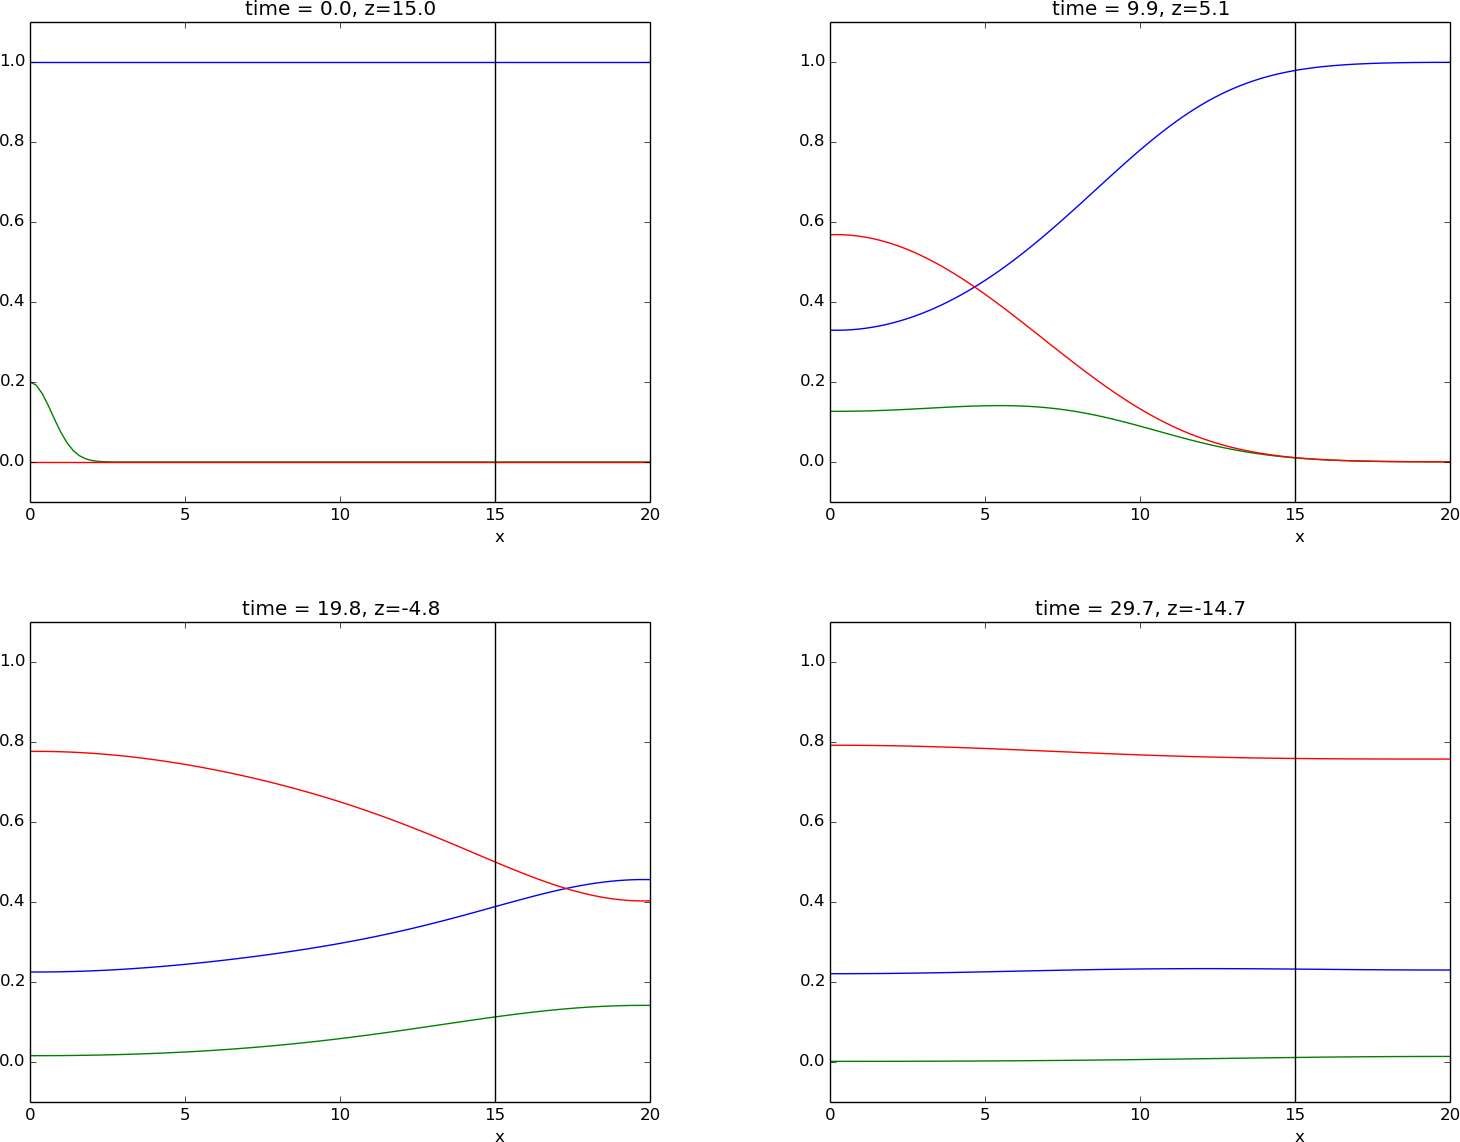
\includegraphics[width=0.8\linewidth]{2_fig/trav_wave_sub.png}}
  \caption{
  \label{fig:1D_sub} The system (\ref{eq:ord_diff_sys}. A gaussian curve with height 0.2 placed on the left side. This causes an epidemic wave controlled by the parameter $\lambda=0.5$. The size is measured at point $x=15$ and can be seen in figure (\ref{fig:1D_tw}).
  }
\end{figure}
%\clearpage % flush figures fig:1D_sub



\begin{figure}[ht]
  \centerline{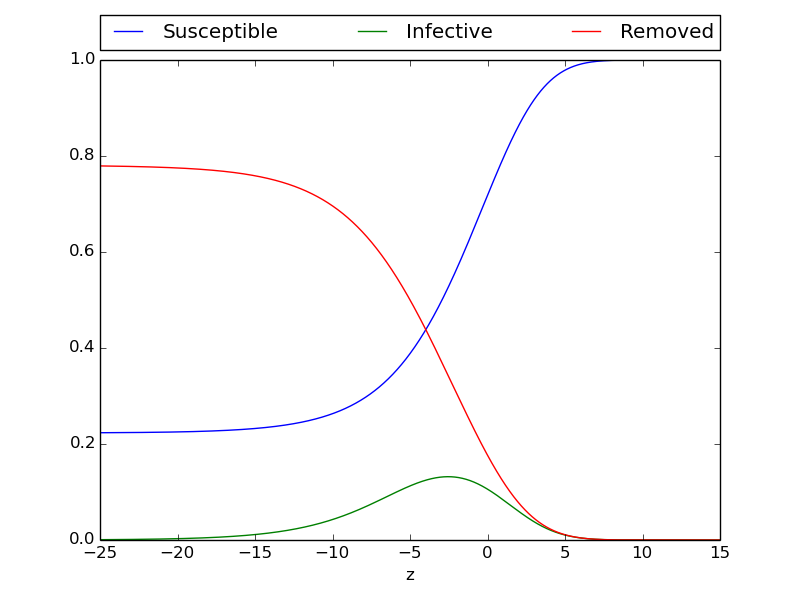
\includegraphics[width=0.9\linewidth]{2_fig/epidemic_wave_z_lambda_0_5.png}}
  \caption{
  \label{fig:1D_tw} This shows the travelling wave measures at at $x=15$ in figure(\ref{fig:1D_sub})
  }
\end{figure}
%\clearpage % flush figures fig:1D_tw




\vspace{3mm}


The \emph{Infective} group in Eq.(\ref{eq:ord_diff_sys}) can be linearised when $z\rightarrow \infty$. This leads to $S\rightarrow 1$ and $I \rightarrow 0$. The result then become 
\begin{equation}
	I'' + cI' + I(S-\lambda) \approx 0 
\end{equation}
This can be found by
\begin{equation}
I(z) \propto \exp\left[(-c \pm {c^2 -4(1-\lambda)}^{1/2})z/2\right]
\end{equation}
Since it is required that $I(z)\rightarrow 0$ and $I(z) > 0$, oscillations around 0 must be prevented. If a travelling wave exist, it has to satisfy
\begin{equation}
	c \geq 2(1-\lambda)^{1/2}, \lambda < 1
\end{equation}
If $\lambda > 1$, no travelling wave will exist. Then the disease will die out. The terms defined in Eq.(\ref{eq:constants_nondimensional}) will give the threshold conditions,
\begin{equation}
	\lambda = \frac{a}{rS_0} < 1
\end{equation}
This is the same value that was given for the ODE model in the previously chapter.
\subsection{Verifying the solution}
To verify the implementation of the solution, a couple of tests can be done one the system in Eq.(\ref{eq:simple_non_PDE}). The system will be tested with a constant solution and a manufactured solution.   

\subsection{Constant solution}
A constant solution uses preproduced constant values for the concentrations $S$, $I$ and $R$. These can be replaced by $S = C_s,I=C_i,R=C_r$. The value of $C_i$ can only be 0 in Eq.(\ref{eq:simple_non_PDE}). This results in a poor test where several bugs can escape. The system can be expanded by adding a term $\beta R$ to the \emph{Susceptible} group and subtracting the same term from the \emph{Removed} group. Then all three values can be tested. The system will then look like this: 
\begin{equation} \label{eq:simple_non_PDE2}
	\begin{aligned}
	\frac{\partial S}{\partial t} &= -IS + \beta R + \frac{\partial^2 S}{\partial x^2},\\
	\frac{\partial I}{\partial t} &= IS- \lambda I + \frac{\partial^2 I}{\partial x^2},\\
	\frac{\partial R}{\partial t} &= \lambda I - \beta R + \frac{\partial^2 R}{\partial x^2},
	\end{aligned}
\end{equation}
By deriving Eq.(\ref{eq:simple_non_PDE2}), the following system Eq.(\ref{eq:constant_PDE}) has to be solved
\begin{equation} \label{eq:constant_PDE}
	\begin{aligned}
	C_iC_s &= \beta C_r \\
	C_iC_s &= \lambda C_i \\
	\lambda C_i &= -\beta C_r 
	\end{aligned}
\end{equation}
The values $\beta$ and $\lambda$ are based on the constants $C_s,C_i,C_r$, which can be chosen freely. Here they are set to $C_s = 1.2,C_i=0.8,C_r=0.6$. This results in $\lambda= C_s = 1.2$ and $\beta= \frac{C_s C_i}{C_r}=1.6$. A test is made in python and can be seen below.

\begin{Verbatim}[numbers=none,fontsize=\fontsize{9pt}{9pt},baselinestretch=0.95]
def test_constant_solution():
    """
    Test problem where u=u_const is the exact solution, to be
    reproduced (to machine precision) by any relevant method.
    """
    def exact_solution(t):
        return C_s,C_i,C_r
    
    def lam(t,x):
        return C_s

    def beta(t,x):
        return (C_s*C_i)/float(C_r)

    #Constant values
    C_s = 1.2
    C_i = 0.8
    C_r = 0.6
    
    #lam = C_s
    #beta = (lam*C_i)/float(C_r)
    
    T = 2; Nt = 200
    X = 20; Nx = 40
    S_1 = np.ones(Nx+3)*C_s
    I_1 = np.ones(Nx+3)*C_i
    R_1 = np.ones(Nx+3)*C_r
    
    t,x,S,I,R = simple_PDE(T,Nx,Nt,X,lam,beta,S_1,I_1,R_1)
    
    S_e,I_e,R_e = exact_solution(t)
    difference = abs(S_e - S).max()  # max deviation
    tol = 1E-14
    assert difference < tol

    difference = abs(I_e - I).max()  # max deviation
    tol = 1E-14
    assert difference < tol

    difference = abs(R_e - R).max()  # max deviation
    tol = 1E-14
    assert difference < tol
\end{Verbatim}

The test was run with no error, and the three constant values were produced correctly. This test is not good enough to qualify the program alone, however an error here would result in a large error in the program. 
\subsection{Manufactured solution}
By constructing a function to each equation in the Eq.(\ref{eq:simple_non_PDE}), a manufactured solution can be created. Here $S$,$I$ and $R$ are pre produced. The system will be
\begin{equation} \label{eq:simple_non_PDE3}
	\begin{aligned}
	\frac{\partial S}{\partial t} &= -IS + \frac{\partial^2 S}{\partial x^2}+f(x,t),\\
	\frac{\partial I}{\partial t} &= IS- \lambda I + \frac{\partial^2 I}{\partial x^2}+g(x,t),\\
	\frac{\partial R}{\partial t} &= \lambda I + \frac{\partial^2 R}{\partial x^2}+h(x,t),
	\end{aligned}
\end{equation}
where $f$, $g$ and $h$ are functions to achieve the expected results for $S$, $I$ and $R$. In this case the functions will be:
\begin{equation}
	\begin{aligned}
	f(x,t) = \frac{\partial S}{\partial t} + IS - \frac{\partial^2 S}{\partial x^2}\\
	g(x,t) = \frac{\partial I}{\partial t} - IS + \lambda I - \frac{\partial^2 I}{\partial x^2}\\
	h(x,t) = \frac{\partial R}{\partial t} -\lambda I - \frac{\partial^2 R}{\partial x^2},
	\end{aligned}
\end{equation}
When choosing the expected function for the groups, it is important that the boundary conditions from Eq.(\ref{eq:boundary_initial}) is fulfilled.
\begin{equation}
    u_x(0,t) = u_x(X,t) = 0
\end{equation}
The quantities have been set to:
\begin{equation}
	\begin{aligned}
    S(x,t) = cos(\frac{\pi}{X}x)t\\
    I(x,t) = cos(\frac{\pi}{X}x)t\\
    R(x,t) = cos(\frac{\pi}{X}x)t
	\end{aligned}
\end{equation}
Now \Verb!sympy! can be used to do the calculations for the three functions $f$, $g$ and $h$. The program can be seen in the Appendix. This results in the following equations seen in Eq.(\ref{eq:manu_func}) 
\begin{equation} \label{eq:manu_func}
	\begin{aligned}
	f(x,t) &= (t^2\cos(\frac{\pi}{X} x) + (\frac{\pi}{X})^2t + 1)\cos(\frac{\pi}{X} x)\\
	g(x,t) &= (\lambda t - t^2\cos(\frac{\pi}{X} x) + (\frac{\pi}{X})^2t + 1)\cos(\frac{\pi}{X} x)\\
	h(x,t) &= (-\lambda t + (\frac{\pi}{X})^2t + 1)\cos(\frac{\pi}{X} x)
	\end{aligned}
\end{equation}
A similar test made for the constant solution can be used here. While the constant test expected a difference on machine precision, this is not the case here. In this test, an expected convergence rate can be measured. The following manufactured test will be

\begin{Verbatim}[numbers=none,fontsize=\fontsize{9pt}{9pt},baselinestretch=0.95]
def test_manufactured_solution(T,Nt,X,Nx):
    
    def exact_solution_S(t,x):
        return np.cos(np.pi*x)*t

    def exact_solution_I(t,x):
        return np.cos(np.pi*x)*t

    def exact_solution_R(t,x):
        return np.cos(np.pi*x)*t


    def beta(t,x):
        return exact_solution_S(t,x)*exact_solution_I(t,x)/exact_solution_R(t,x)
   
    def f(t,x):
        return (t**2*np.cos(np.pi*x) + (np.pi/float(X))**2*t + 1)*np.cos(np.pi*x) 

    def g(t,x):
        return (lam*t - t**2*np.cos(np.pi*x) + (np.pi/float(X))**2*t + 1)*np.cos(np.pi*x)

    def h(t,x):
        return (-lam*t + (np.pi/float(X))**2*t + 1)*np.cos(np.pi*x)
        

    dx = X/float(Nx)
    dt = T/float(Nt)
    S_1 = exact_solution_S(0,np.linspace(0-dx,X+dx,Nx+3))
    I_1 = exact_solution_I(0,np.linspace(0-dx,X+dx,Nx+3))
    R_1 = exact_solution_R(0,np.linspace(0-dx,X+dx,Nx+3))
     
    t,x,S,I,R = simple_PDE(T,Nx,Nt,X,lam,beta,S_1,I_1,R_1,f,g,h)
    S_e = exact_solution_S(t[-1],x)
    I_e = exact_solution_I(t[-1],x)
    R_e = exact_solution_R(t[-1],x)
    
    difference_S = abs(S_e - S).max()  # max deviation
    difference_I = abs(I_e - I).max()  # max deviation
    difference_R = abs(R_e - R).max()  # max deviation

    return difference_S,difference_I,difference_R
\end{Verbatim}

\subsection{Convergence rate}
The program can be controlled by checking the convergence rate. The error term  for this equation can be described as  
\begin{equation} \label{eq:error}
    \epsilon = C_x\Delta x^2 + C_t \Delta t
\end{equation}
With Eq.(\ref{eq:error}), the expected convergence rate can be found for both $\Delta x$ and $\Delta t$. To be able to separate the $\Delta$s, the other value has to be close to eliminated. To study the value $\Delta x$, the following term has to be fullfilled: $\Delta t \ll \Delta x$. This will lead to $C_t\Delta t \approx 0$, and the error term for $\Delta x$ can be found. The opposite thing can  be done for $\Delta t$. A table for the error is produced for different values for $\Delta t = 0.05$ and $\Delta x=0.1$.

\label{table:error_numbers}

\begin{quote}
\begin{tabular}{ccccc}
\hline
\multicolumn{1}{c}{  } & \multicolumn{1}{c}{ $\Delta x$ } & \multicolumn{1}{c}{ $\frac{\Delta x}{2}$ } & \multicolumn{1}{c}{ $\frac{\Delta x}{4}$ } & \multicolumn{1}{c}{ $\frac{\Delta x}{8}$ } \\
\hline
$\Delta t     $       & 9.9E-3     & -                    & -                    & -                    \\
$\frac{\Delta t}{4} $ & 9.9E-3     & 2.5E-3               & -                    & -                    \\
$\frac{\Delta t}{8} $ & 9.9E-3     & 2.5E-3               & 6.1E-4               & -                    \\
$\frac{\Delta t}{16}$ & 9.9E-3     & 2.5E-3               & 6.1E-4               & 1.5E-4               \\
\hline
\end{tabular}
\end{quote}

\noindent
% 0.00988006143376,0.00246039081619,-,-
% 0.00988361769746,0.00246127510994,0.000614719954035
% 0.00988450717896,0.00246149628689,0.000614775174047,0.000153656409034

\subsection{The spatial error}
The Tab.(\ref{table:error_numbers}) gives information about the error when $\Delta t$ and $\Delta x$ are reduced. By studying the row where $\Delta t/16$, the $C_t \Delta t$ can be seen as close to negligible in Eq.(\ref{eq:error}). The error can be expressed 
\begin{equation}
    \epsilon \propto \Delta x^r
\end{equation}
The value is expected to be $r=2$, since centered difference is used in the spatial discretization. By comparing the error for different $\Delta x$, the convergence rate, $r$, can be expressed, 
\begin{equation} \label{eq:conv_rate}
 r_{12} \simeq \frac{\log(\epsilon_1/\epsilon_2)}{\log(\Delta x_1/\Delta x_2)}
\end{equation}
Since the table above has four different error values, these can be used to give three different convergence rates. $\Delta x_1 = \Delta x, \Delta x_2 = \Delta x/2...$. The same notation has been used for the different error values, $\epsilon$.

\begin{quote}
\begin{tabular}{cccc}
\hline
\multicolumn{1}{c}{  } & \multicolumn{1}{c}{ $\epsilon_1/\epsilon_2$ } & \multicolumn{1}{c}{ $\epsilon_2/\epsilon_3$ } & \multicolumn{1}{c}{ $\epsilon_3/\epsilon_4$ } \\
\hline
r & 2.0056                  & 2.0014                  & 2.0004                  \\
\hline
\end{tabular}
\end{quote}

\noindent
Here the rate goes towards 2, and a 2.order convergence rate seems to be fulfilled.
\subsection{The temporal error}
The temporal error is hard to find since the \emph{Stability criteria} expects $\Delta t$ to fulfill the criteria in Eq.(\ref{eq:stability_cr}) to avoid oscillations.
\begin{equation} \label{eq:stability_cr}
 \Delta t \leq \frac{\Delta x^2}{2}
\end{equation}
As a result, $\Delta x \ll \Delta t$ is impossible, because this only leads to an unstable solution. By looking at the column for $\frac{\Delta x}{8}$, the only stable solution is for $\frac{\Delta t}{16}$. Therefore the technique used for the spatial error cannot be used here. 

\subsection{Travelling wave in 2D}
The Eq.(\ref{eq:simple_non_PDE}) can be discretized for a 2D area. This is more realistic when simulating a geographic spread of an epidemic disease. The non dimensional system  can be discretized with Forward Euler in time and centered difference in space
\begin{equation} \label{eq:SIR_disc}
	\begin{aligned}
    \frac{S^{n+1}_{i,j}-S^n_{i,j}}{\Delta t} &= -I^{n}_{i,j}S^{n}_{i,j} + \left(\frac{S^{n}_{i-1,j}-2S^{n}_{i,j}+S^{n}_{i+1,j}}{\Delta x^2}+\frac{S^{n}_{i,j-1}-2S^{n}_{i,j}+S^{n}_{i,j+1}}{\Delta y^2}\right) \\
    \frac{I^{n+1}_{i,j}-I^n_{i,j}}{\Delta t} &= I^{n}_{i,j}S^{n}_{i,j} -\lambda I^{n}_{i,j} + \left(\frac{I^{n}_{i-1,j}-2I^{n}_{i,j}+I^{n}_{i+1,j}}{\Delta x^2}+\frac{I^{n}_{i,j-1}-2I^{n}_{i,j}+I^{n}_{i,j+1}}{\Delta y^2}\right) \\
    \frac{R^{n+1}_{i,j}-R^n_{i,j}}{\Delta t} &= \lambda I^{n}_{i,j}+\left(\frac{R^{n}_{i-1,j}-2R^{n}_{i,j}+R^{n}_{i+1,j}}{\Delta x^2}+\frac{R^{n}_{i,j-1}-2R^{n}_{i,j}+R^{n}_{i,j+1}}{\Delta y^2}\right) 
	\end{aligned}
\end{equation}
The known values can be placed on the right side. The system will then be
\begin{equation}
	\begin{aligned}
    S^{n+1}_{i,j} &= S^{n}_{i,j}+\Delta t\left(-I^{n}_{i,j}S^{n}_{i,j} + \left(\frac{S^{n}_{i-1,j}-2S^{n}_{i,j}+S^{n}_{i+1,j}}{\Delta x^2}+\frac{S^{n}_{i,j-1}-2S^{n}_{i,j}+S^{n}_{i,j+1}}{\Delta y^2}\right)\right) \\
    I^{n+1}_{i,j} &= I^{n}_{i,j}+\Delta t\left(I^{n}_{i,j}S^{n}_{i,j} -\lambda I^{n}_{i,j} + \left(\frac{I^{n}_{i-1,j}-2I^{n}_{i,j}+I^{n}_{i+1,j}}{\Delta x^2}+\frac{I^{n}_{i,j-1}-2I^{n}_{i,j}+I^{n}_{i,j+1}}{\Delta y^2}\right)\right) \\
    R^{n+1}_{i,j} &= R^{n}_{i,j}+\Delta t\left(\lambda I^{n}_{i,j}+\left(\frac{R^{n}_{i-1,j}-2R^{n}_{i,j}+R^{n}_{i+1,j}}{\Delta x^2}+\frac{R^{n}_{i,j-1}-2R^{n}_{i,j}+R^{n}_{i,j+1}}{\Delta y^2}\right)\right) 
	\end{aligned}
\end{equation}
This results in an explicit system, which is easy to code. It consists of known values on the right side and only one unknown value on the left side.
\subsection{A gaussian wave}
In the PDE system for the 1D equation, a Gaussian quantity of infected humans was placed on the left side in the initial value. This resulted in a wave of \emph{Infected} spreading along the x-axis. A similar procedure can be done for the 2D simulation. A couple of simulations have been produced for the 2D system. The first simulation is calculated with a Gaussian function along the points(0,y) for the \emph{Infected} group at initial time. The second simulation has placed the Gaussian function at point(0,0) for the \emph{Infected} group at initial value. Both simulations can be seen in the Appendix.  


\vspace{3mm}




\vspace{3mm}


The size of the epidemic wave can be measured and compared by studying the travelling wave at a certain point. In these two 2D simulations in Fig.(\ref{fig:2D_trav_wave}), the wave are measured in the point (15,15), while the travelling wave in the 1D simulation was measured at point(15). 


\begin{figure}[ht]
  \centerline{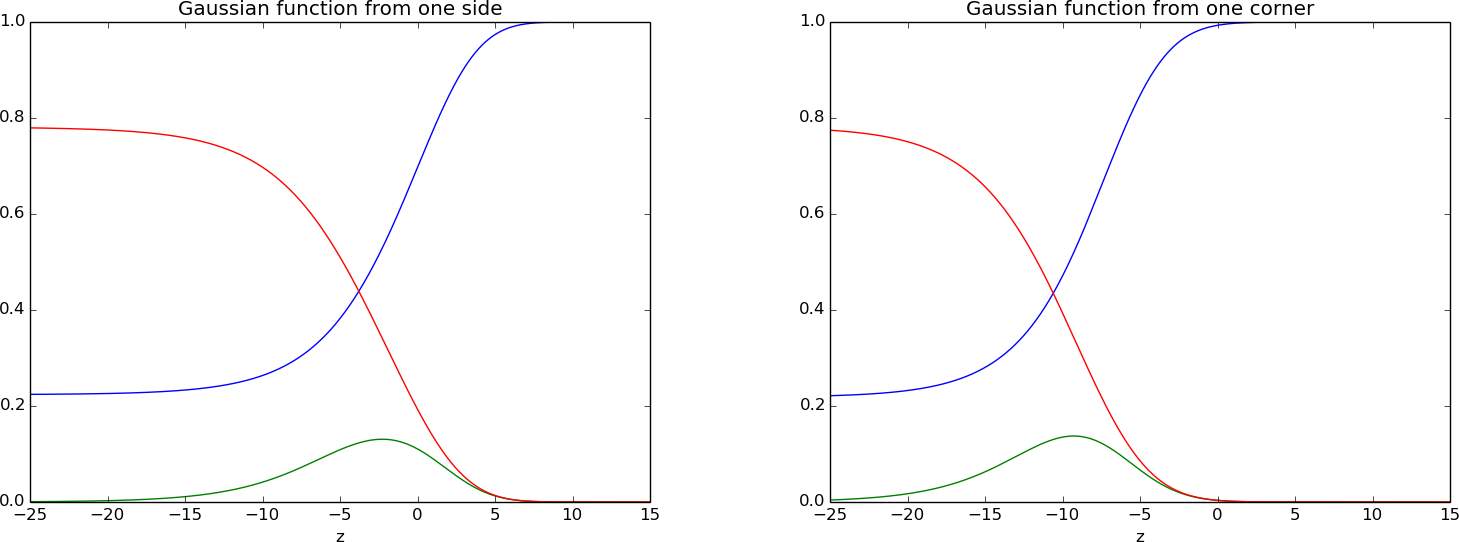
\includegraphics[width=0.8\linewidth]{2_fig/Trav_wave_2D.png}}
  \caption{
  \label{fig:2D_trav_wave} Travelling wave measured at point (15,15) with two different initial values for the \emph{Infected} group. I:The initial value is set as a Gaussian line along (0,y).II:The initial value is set as a Gaussian point (0,0).
  }
\end{figure}
%\clearpage % flush figures fig:2D_trav_wave




\vspace{3mm}




\vspace{3mm}


The shapes of the two travelling waves in Fig.(\ref{fig:2D_trav_wave}) are similar. The only difference is the time when the wave occurs. The plot for 1D wave in Fig.(\ref{fig:1D_tw}) has the same shape. With a closer study, the area under the function can be measured in all three cases. The result can be seen in Tab.(\ref{table:wave_values})   

% 1D
% 1.4340793845
% 1.43143259034 dt = $1\cdot10^{-3}$, dx = 0.05
% 1.43195870243 dt = 0.0002, dx^2 = 0.000625
% 2D wave line:
% 1.43345609926 dt =0.0004, dx^2 =  0.0016
% 2D wave point:
% 1.43352971688

\label{table:wave_values}

\begin{quote}
\begin{tabular}{ccc}
\hline
\multicolumn{1}{c}{ 1D wave } & \multicolumn{1}{c}{ 2D wave line } & \multicolumn{1}{c}{ 2D wave point } \\
\hline
1.43    & 1.43         & 1.43          \\
\hline
\end{tabular}
\end{quote}

\noindent
The area in all three simulations approach the same area when $\Delta t$ and $\Delta x$ are reduced. The size and shape will not change by  expanding the system from 1D to 2D. However, by studying Fig.(\ref{fig:2D_trav_wave}), one can see that the wave occurs at different times. This is caused by the distance from the start position for the Gaussian wave. The first subplot that starts with a Gaussian function along the $x=0$ axis gets a wave from the \emph{Infected} group that flows along the x axis. This can be seen as a wave on the beach. Everyone that have the same distance from the ocean will be hit simultaneously. The travelling wave for the 1D simulation and the first subplot occurs at the same time, because they are measured at the same distance from the starting point. The last plot is also measured at (15,15), but occurs later. Since the wave starts at point (0,0), the distance to (15,15) is 21.21. This means that the wave will reach the point 6.21 time steps later. This is a reasonable conclusion based on the plot.    

\paragraph{Change in initial flow.}
By increasing the initial wave of the \emph{Infected} group, the initial value of \emph{Infected} can be studied. The simulation is run with the same parameters as for the three simulations above and the only difference is the initial value for the \emph{Infected} group. The Gaussian wave of \emph{Infected} is placed at point(0,0) as for subplot II in Fig.(\ref{fig:2D_trav_wave}). The simulation can be seen in Fig.(\ref{fig:initial_value}).  
% Volume ordinary = 0.3141592653589793
% Volume extreme = 157.07963267948966
% Volume under graph 1.43345609926


\begin{figure}[ht]
  \centerline{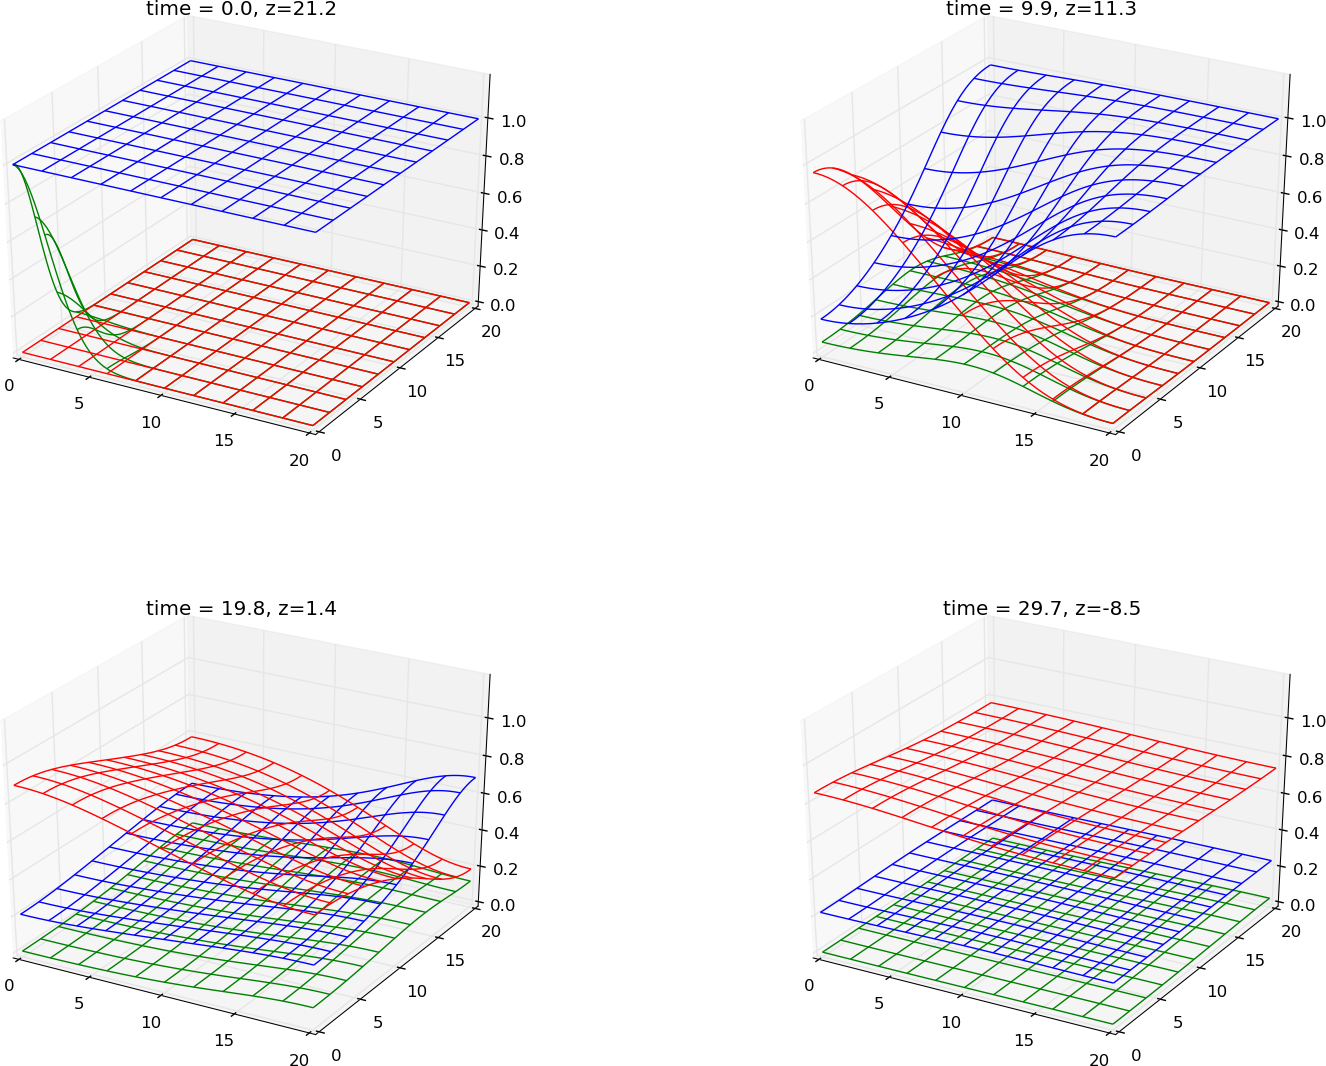
\includegraphics[width=0.8\linewidth]{2_fig/2D_initial_variable_sub.png}}
  \caption{
  \label{fig:initial_value} A major flow of \emph{Infected} spread outwards in the field. After a certain time, the wave has passed the area and the number in each group stabilized.
  }
\end{figure}
%\clearpage % flush figures fig:initial_value




\vspace{3mm}




\vspace{3mm}


The size and shape can be compared by measuring the travelling wave at point(15,15). The travelling wave for this simulation can be seen in Fig.(\ref{fig:initial_trav_wave}) and the area for the travelling wave is measured to 1.43, which is similar to the three other simulations.


\begin{figure}[ht]
  \centerline{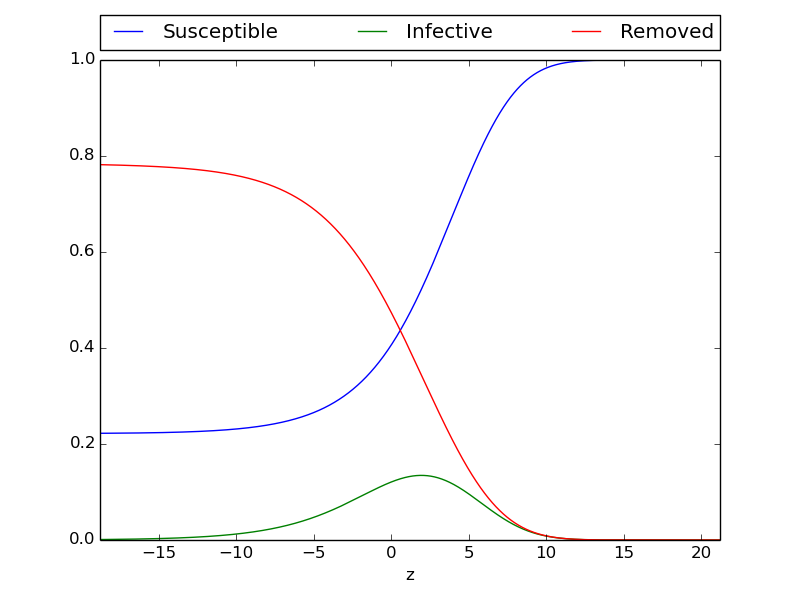
\includegraphics[width=0.8\linewidth]{2_fig/TW_2D_initial_z_lambda_0_5.png}}
  \caption{
  \label{fig:initial_trav_wave} The travelling wave with a major increase of \emph{Infected} at the initial time.
  }
\end{figure}
%\clearpage % flush figures fig:initial_trav_wave




\vspace{3mm}




\vspace{3mm}


The size of the travelling  wave will not be affected by changing the value of the \emph{Infected} group. However there is a difference in the time when the wave occurs. In the simulation where the initial value is higher, the travelling wave reaches the measuring point (15,15) earlier. This can be explained by the idea of a ball dropped from a large height. If the ball is released or thrown to the ground, it will only affect the acceleration of the ball, not the terminal velocity. After a certain time the released ball and the thrown ball will reach the same maximum speed. This is the case for the speed of the travelling wave. 
\paragraph{Change in lambda.}
The one thing that affects the speed and size, is the $\lambda$ variable in the PDE system(\ref{eq:simple_non_PDE}). This $\lambda$ is a combination of $a$, which controls deaths among the \emph{Infected} group, $r$, which controls the number from the \emph{Susceptible} group that gets infected in meetings between the \emph{Infected} and \emph{Susceptible} groups. The last parameter in $\lambda$ is the concentration of Susceptible, $S_0$. By changing this parameter, the travelling wave will change in both size and shape. In Fig.(\ref{fig:change_lambda}), the simulation is run with four different values of $\lambda$.


\begin{figure}[ht]
  \centerline{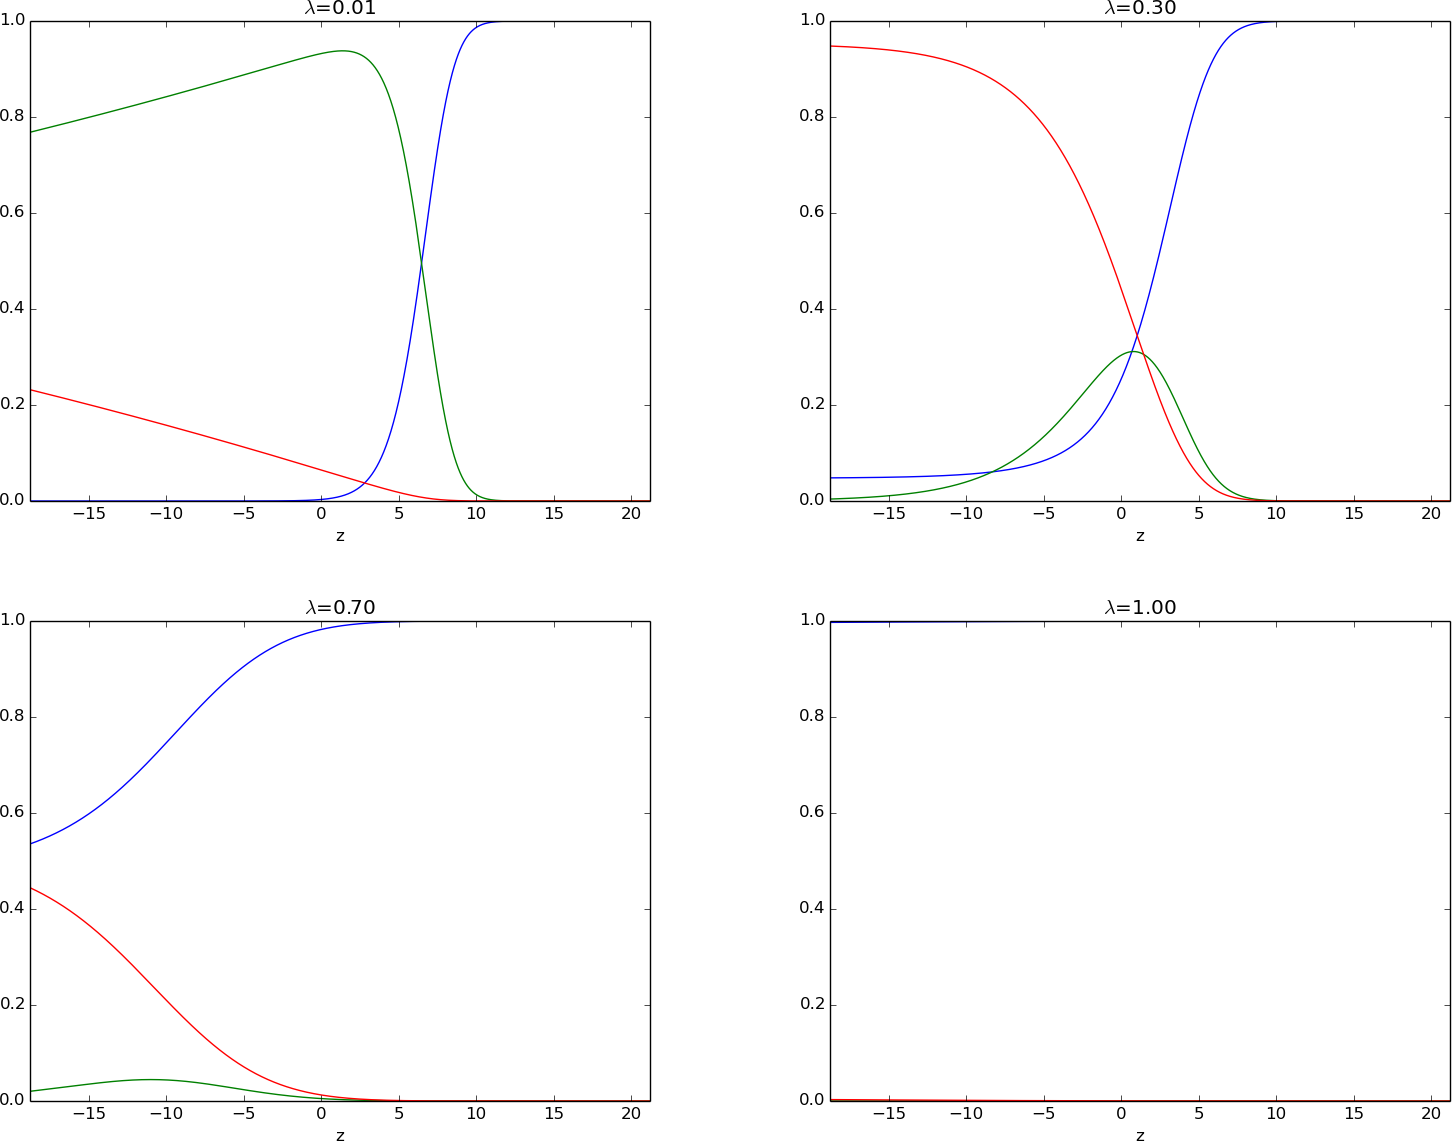
\includegraphics[width=0.9\linewidth]{2_fig/2D_lambda_variable.png}}
  \caption{
  \label{fig:change_lambda} The travelling wave simulated with $\lambda$ values in the range of 0.01 to 1.
  }
\end{figure}
%\clearpage % flush figures fig:change_lambda




\vspace{3mm}




\vspace{3mm}


To understand the results in Fig.(\ref{fig:change_lambda}), the $\lambda $ function can be studied,
\begin{equation} \label{eq:lambda}
 \lambda =\frac{a}{rS_0},
\end{equation}
A major and aggressive travelling wave is caused when $\lambda \rightarrow 0$. In Fig.(\ref{fig:change_lambda}), $\lambda$ is run with value 0.01 in the first subplot. This results in a travelling wave of \emph{Infected} that eradicates the \emph{Susceptible} group in a short time. The wave starts decreasing when all \emph{Susceptible} are infected. By looking at Eq.(\ref{eq:lambda}),one can see that a small value is caused by a small $a$ compared to $r$ and $S_0$. If $a$ is low, this results in few deaths/immune in the \emph{Infected} group. This means that the \emph{Infected} group will grow and be able to infect even more humans from the \emph{Susceptible} group. The same thing will happen if $r$ is large. A result of a large $r$ will be an aggressive disease that infects  a major part of the population. The same result will happen if $S_0$ is large. Then there are several possible humans to infect. Therefore an outburst of a disease is more critical in a crowded city than in the wilderness, far from other humans.


\vspace{3mm}




\vspace{3mm}


If $\lambda$ increases above 1, the disease will not be able to spread. The number of \emph{Infected} will decrease, since the number in the \emph{Removed} group caused by the \emph{Infected} group is higher than the amount of \emph{Infected} humans from the \emph{Susceptible} group. After a certain time, the number of \emph{Infected} will die out. If $\lambda$ stays at 1, the number of \emph{Infected} will be equal the whole time. 

\section{English Boarding School}
An example from an English boarding school was presented in the previously chapter \emph{Epidemic models} . This example was based on the book from J.D Murray \cite{murray2002mathematical}, and was modeled for an ODE system. A similar result should appear for the PDE system with the same parameter values and a uniform distribution of the groups. The school had 763 students, and one of the students brought a disease back to the school. The following numbers were used for the ODE system in chapter one. $N=763, S_0=762,I_0=1,R_0=0,\rho=202$ and $r = 2.18\cdot 10^{-3}$. 


\vspace{3mm}




\vspace{3mm}


The first simulation is produced with uniform distributed concentration, This is done to verify the implementation. A person is defined as one cubic. The total volume of the whole group is spread over the area. The area is set to be 100 m x 100 m, which results in an average height of $1/10000$ m per person. This is done to get a uniformed distribution. This would of course be more difficult in real life, particularly if the person would be alive. Since the \emph{Infected} group only consists of one person, the total height will be 0.0001 for the whole area. The \emph{Susceptible} group consists of 762 students and the total height at each point will be 0.0762 The simulation can be seen in the Appendix. 


\vspace{3mm}




\vspace{3mm}


The results from subplot I in Fig.(\ref{fig:british_number}) are equal to the results from the ODE system modeled in the previously chapter.This can be seen in Tab.(\ref{table:british_number_table}). This is as expected, since the diffusion term is negligible in this system. The simulation results in a group of separate ODE systems modeled over an area.


\begin{figure}[ht]
  \centerline{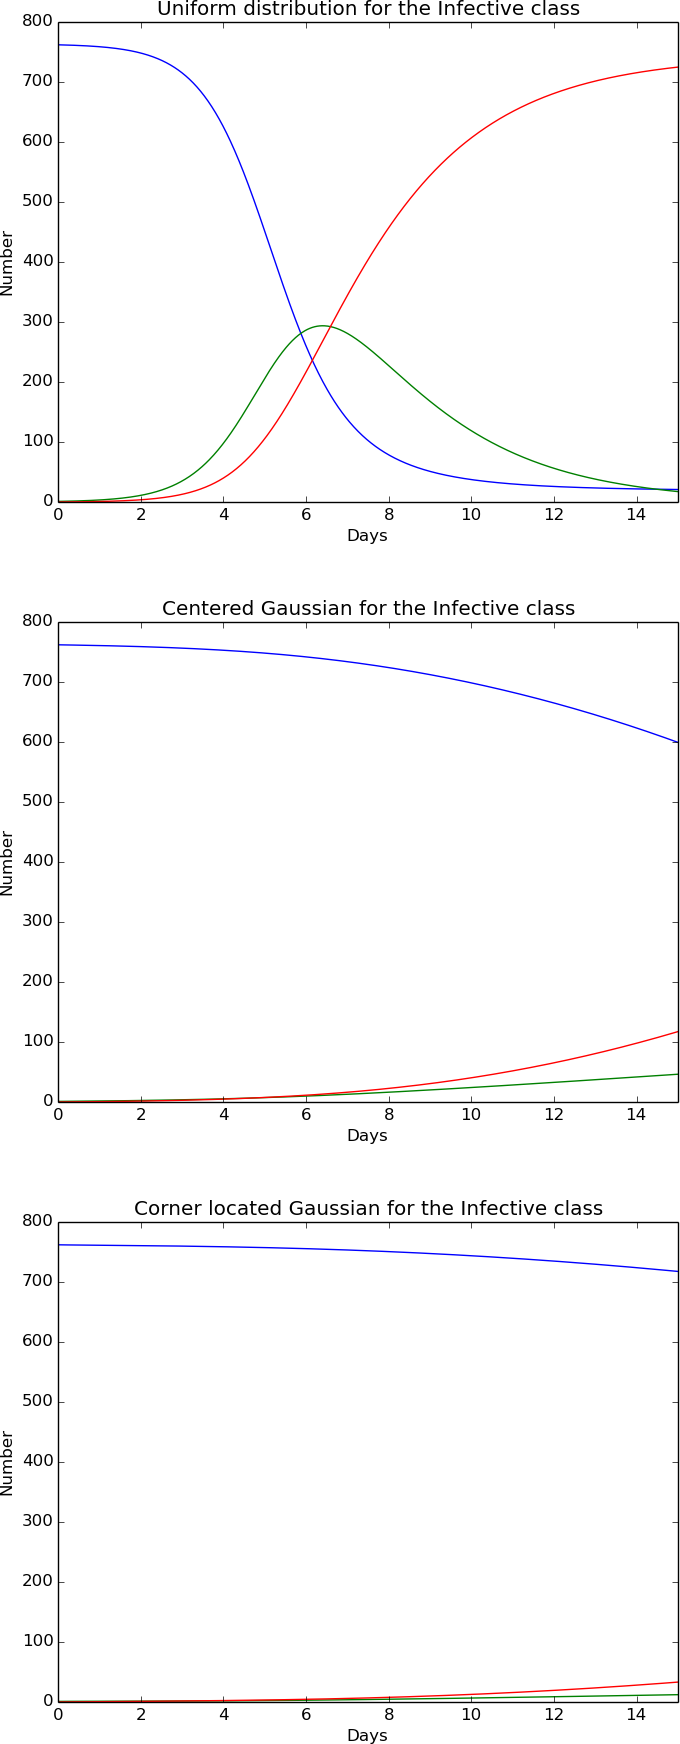
\includegraphics[width=0.6\linewidth]{2_fig/british_number.png}}
  \caption{
  \label{fig:british_number} English Boarding School modeled with three different initial values for the infected student. The amount of students in each group modeled over 15 days. Subplot 1: uniform distribution. Subplot 2: The student is placed as a Gaussian function in center. Subplot 3: The student is placed as a Gaussian function in the corner (0,0).
  }
\end{figure}
%\clearpage % flush figures fig:british_number


\subsection{Maximum concentration of \emph{Infected}}
The maximum concentration of the \emph{Infected} group was found for the ODE system in the previous chapter. The expected value of $\Imax$ was first calculated, and later verified with the numberical solution of the ODE system. The reproduction rate found for the PDE system in Eq.(\ref{eq:reproduction_rate_PDF}) was given by the same parameters as for the ODE system. A similar maximum value is expected from the PDE solution. The maximum value for the \emph{Infected} array is $\Imax=292$ and is similar to the $\Imax$ for the ODE solution. 

A table with the values from the three simulations performed for this English boarding school are compared to ODE system from chapter~\ref{section:ODE_models}.

\label{table:british_number_table}

\begin{quote}
\begin{tabular}{ccccc}
\hline
\multicolumn{1}{c}{  } & \multicolumn{1}{c}{ ODE system } & \multicolumn{1}{c}{ PDE uniform dist } & \multicolumn{1}{c}{ PDE center } & \multicolumn{1}{c}{ PDE corner } \\
\hline
5 Days      & ----------- & ------------------- & ----------- & ----------- \\
\hline
Susceptible & 444.62      & 444.62              & 748.03      & 757.33      \\
Infective   & 209.56      & 209.56              & 7.36        & 2.35        \\
Removed     & 108.82      & 108.82              & 7.60        & 3.32        \\
\hline
10 Days     & ----------- & ------------------- & ----------- & ----------- \\
\hline
Susceptible & 37.59       & 37.59               & 697.71      & 743.58      \\
Infective   & 117.59      & 117.59              & 24.43       & 6.66        \\
Removed     & 607.82      & 607.82              & 40.86       & 12.76       \\
\hline
15 Days     & ----------- & ------------------- & ----------- & ----------- \\
\hline
Susceptible & 21.09       & 21.09               & 597.01      & 717.02      \\
Infective   & 17.30       & 17.30               & 46.96       & 12.37       \\
Removed     & 724.62      & 724.62              & 119.03      & 33.61       \\
\hline
\end{tabular}
\end{quote}

\noindent
% dx = 0.04
% dx^2 = 1.6E-3
% ODE = 1.5E-4

\subsection{Introducing a Gaussian distribution of infected}
An assumption one can make is that a person is not able to be evenly distributed over an area. In this example, with only one infected student at initial time, the chance of being infected increases the closer the \emph{Susceptible} group gets the infected student. The student is represented by a Gaussian function in the middle of the school yard, to see if the position affects the result. The height is set to 1 and the volume of the Gauss function is set to 1 cubic. The simulation can be seen in Fig.(\ref{fig:gauss_sub}) and the total amount of students in each group can be be seen in Fig.(\ref{fig:british_number}).


\begin{figure}[ht]
  \centerline{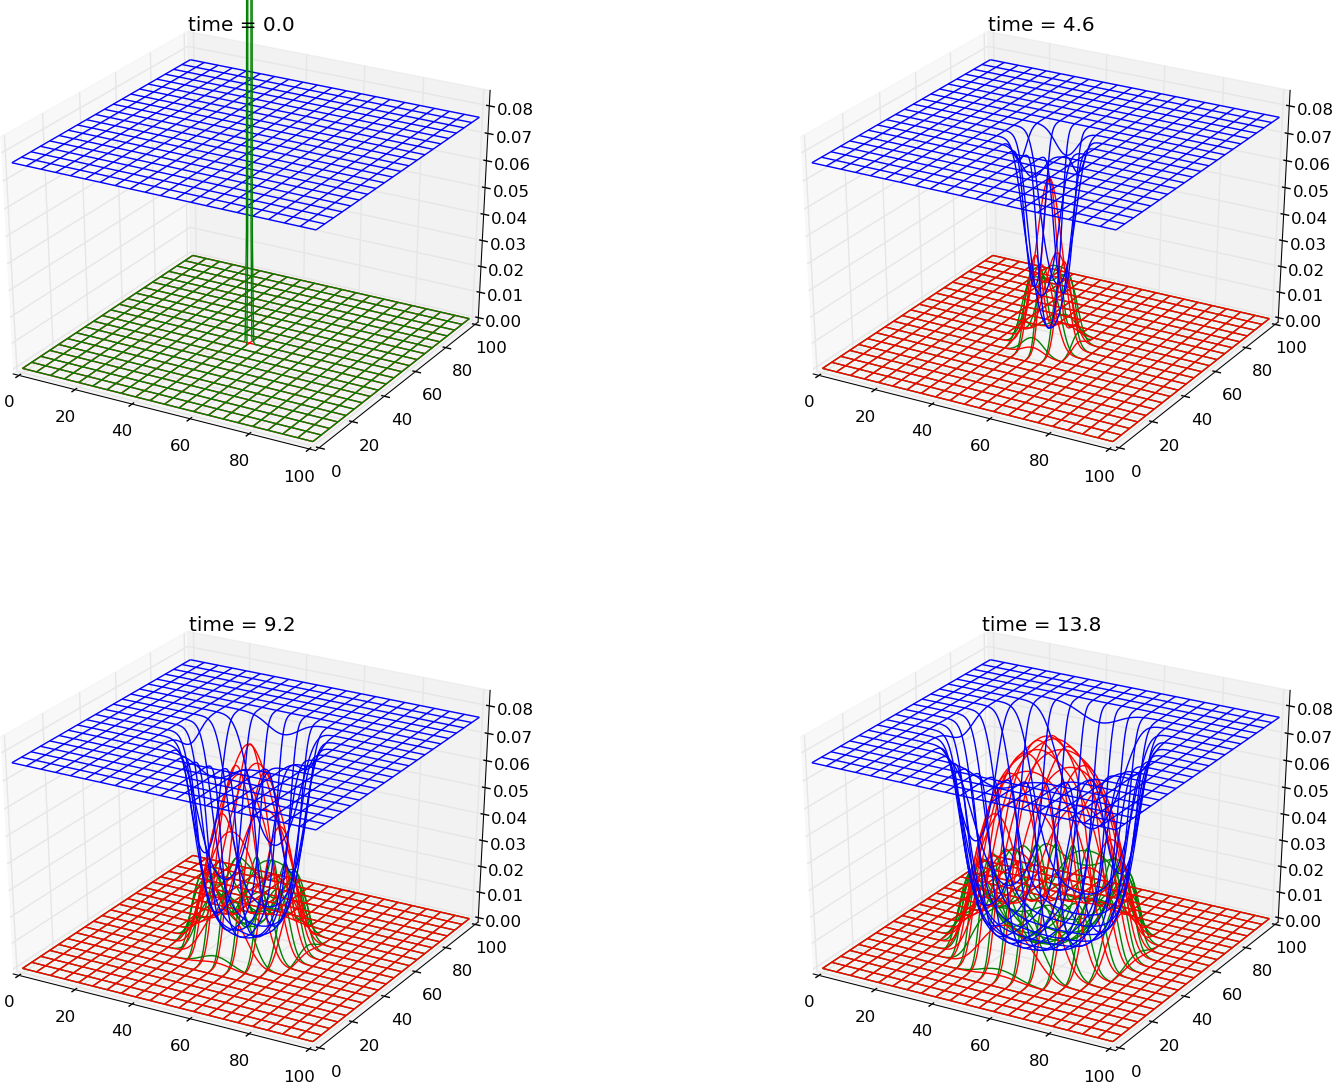
\includegraphics[width=0.8\linewidth]{2_fig/2D_british_school_gauss_sub.png}}
  \caption{
  \label{fig:gauss_sub} The infected student is placed in the center as a Gaussian function at initial time. The height of the Gaussian function is set to 1 m and volume is set to 1 cubic.
  }
\end{figure}
%\clearpage % flush figures fig:gauss_sub




\vspace{3mm}




\vspace{3mm}


The results from the uniform distributed and Gaussian distributed simulations show various results. The initial position of the \emph{Infected} group is the difference between the simulations. This has a major impact. Since the only ones that can be infected by the Gaussian distribution are the students close to the infected student, this restricts the spread of the epidemic. The chance of getting infected in this area is higher. The Fig.(\ref{fig:gauss_sub}) shows that the amount of \emph{Infective} quickly grows in the center, where the infected was placed. Subplot IV in Fig.(\ref{fig:gauss_sub}) shows that the amount from the \emph{Removed} group in the center is close to the maximum of the initial value of \emph{Susceptible}, while the students along the boundary of the schoolyard seem to be unaffected after 15 days. This simulation shows that the position of the \emph{Infected} group has a major role in the simulation.


\vspace{3mm}




\vspace{3mm}


The position of the \emph{Infected} group, here as a Gaussian function, also affects the outcome. Subplot III in Fig.(\ref{fig:british_number}) describes a simulation where the Gaussian function is placed in the corner with position(0,0). The total volume of the function is increased to 4 since only a quarter of the function is placed in the area. Tab.(\ref{table:british_number_table}) shows that the total number of \emph{Infected} is lower than for the centered placed Gaussian function. The infected student is only able to spread the disease to a quarter of the population compared to the infected student in the center. The simulation can be seen in the Appendix.


\vspace{3mm}




\vspace{3mm}


If the simulations are run for a long time, the difference between each group will decrease. After 100 days there will be about 18 students in the \emph{Susceptible} group in the uniform distributed simulation, compared to 25 students in both of the Gaussian simulations. The simulations can be seen in the Appendix.

% !split
\section{Zombiefication}
The previous chapter studied an ODE system designed to calculate the number in the four groups: \emph{Susceptible}, \emph{Infected}, \emph{Zombie} and \emph{Removed} during the five first episodes in the TV series \emph{Walking Dead} Ref.\cite{walking_dead}. The model was based on the model from Langtangen, Mardal and Røtnes Ref.\cite{zombie-math}, with an extra term in the \emph{counter attack} phase. The ODE system from the chapter \emph{Epidemic models} can be expanded with a diffusion term in each group to make a PDE system. This can be seen in Eq.(\ref{eq:seland_model_PDE})  
\begin{equation} \label{eq:seland_model_PDE}
	\begin{aligned} 
	\frac{\partial S}{\partial t} &= \Sigma -(\beta+\mu \omega(t))SZ - \delta_SS +D_s\nabla^2 S \\
	\frac{\partial I}{\partial t} &= (\beta+\mu \omega(t))SZ - \varrho I - \delta_II+D_i\nabla^2 I \\
	\frac{\partial Z}{\partial t} &= \varrho I- (\alpha+\omega(t))SZ + \zeta R+D_z\nabla^2 Z \\
	\frac{\partial R}{\partial t} &= \delta_SS +\delta_II -\zeta R + (\alpha+\omega(t))SZ+D_r\nabla^2 R 
	\end{aligned}
\end{equation}
The Eq.(\ref{eq:seland_model_PDE}) can be solved numerically by discretization. Forward Euler is used for the time derivative and centered difference for the space derivative. This is solved with the same technique as for the SIR model(\ref{eq:SIR_disc}). The system can be seen in Eq.(\ref{eq:SIZR_disc})
\begin{equation} \label{eq:SIZR_disc}
	\begin{aligned}
    \frac{S^{n+1}_{i,j}-S^n_{i,j}}{\Delta t} &= \Sigma - (\beta+\mu \omega(t))S^{n}_{i,j}Z^{n}_{i,j}- \delta_S S^{n}_{i,j} \\
        &+D_s\left(\frac{S^{n}_{i-1,j}-2S^{n}_{i,j}+S^{n}_{i+1,j}}{\Delta x^2}+\frac{S^{n}_{i,j-1}-2S^{n}_{i,j}+S^{n}_{i,j+1}}{\Delta y^2}\right) \\
    \frac{I^{n+1}_{i,j}-I^n_{i,j}}{\Delta t} &= (\beta+\mu \omega(t))S^{n}_{i,j}Z^{n}_{i,j}-\varrho I^{n}_{i,j}- \delta_I I^{n}_{i,j} \\
        &+D_i\left(\frac{I^{n}_{i-1,j}-2I^{n}_{i,j}+I^{n}_{i+1,j}}{\Delta x^2}+\frac{I^{n}_{i,j-1}-2I^{n}_{i,j}+I^{n}_{i,j+1}}{\Delta y^2}\right) \\
    \frac{Z^{n+1}_{i,j}-Z^n_{i,j}}{\Delta t} &= \varrho I^{n}_{i,j}-(\alpha+\omega(t))S^{n}_{i,j}Z^{n}_{i,j}+ \zeta R^{n}_{i,j} \\
        &+D_z\left(\frac{Z^{n}_{i-1,j}-2Z^{n}_{i,j}+Z^{n}_{i+1,j}}{\Delta x^2}+\frac{Z^{n}_{i,j-1}-2Z^{n}_{i,j}+Z^{n}_{i,j+1}}{\Delta y^2}\right) \\
    \frac{R^{n+1}_{i,j}-R^n_{i,j}}{\Delta t} &= \delta_S S^{n}_{i,j}+\delta_I I^{n}_{i,j}-\zeta R^{n}_{i,j}+(\alpha+\omega(t))S^{n}_{i,j}Z^{n}_{i,j} \\
        &+D_r\left(\frac{R^{n}_{i-1,j}-2R^{n}_{i,j}+R^{n}_{i+1,j}}{\Delta x^2}+\frac{R^{n}_{i,j-1}-2R^{n}_{i,j}+R^{n}_{i,j+1}}{\Delta y^2}\right) 
	\end{aligned}
\end{equation}
By setting the unknown to the left, the following system in Eq.(\ref{eq:SIZR_disc2}) can be solved: 
\begin{equation}\label{eq:SIZR_disc2}
	\begin{aligned}
    S^{n+1}_{i,j} &= S^n_{i,j} + \Delta t \Bigl( \Sigma - (\beta+\mu \omega(t))S^{n}_{i,j}Z^{n}_{i,j}- \delta_S S^{n}_{i,j} \\
        &+ D_s\left(\frac{S^{n}_{i-1,j}-2S^{n}_{i,j}+S^{n}_{i+1,j}}{\Delta x^2}+\frac{S^{n}_{i,j-1}-2S^{n}_{i,j}+S^{n}_{i,j+1}}{\Delta y^2}\right)\Bigr) \\
    I^{n+1}_{i,j} &= I^n_{i,j} + \Delta t \Bigl((\beta+\mu \omega(t))S^{n}_{i,j}Z^{n}_{i,j}-\varrho I^{n}_{i,j}- \delta_I I^{n}_{i,j} \\
        &+ D_i\left(\frac{I^{n}_{i-1,j}-2I^{n}_{i,j}+I^{n}_{i+1,j}}{\Delta x^2}+\frac{I^{n}_{i,j-1}-2I^{n}_{i,j}+I^{n}_{i,j+1}}{\Delta y^2}\right)\Bigr) \\ 
    Z^{n+1}_{i,j} &= Z^n_{i,j} +\Delta t \Bigl( \varrho I^{n}_{i,j}-(\alpha+\omega(t))S^{n}_{i,j}Z^{n}_{i,j}+ \zeta R^{n}_{i,j} \\
        &+D_z\left(\frac{Z^{n}_{i-1,j}-2Z^{n}_{i,j}+Z^{n}_{i+1,j}}{\Delta x^2}+\frac{Z^{n}_{i,j-1}-2Z^{n}_{i,j}+Z^{n}_{i,j+1}}{\Delta y^2}\right)\Bigr) \\
    R^{n+1}_{i,j} &= R^n_{i,j} +\Delta t \Bigl(\delta_S S^{n}_{i,j}+\delta_I I^{n}_{i,j}-\zeta R^{n}_{i,j}+(\alpha+\omega(t))S^{n}_{i,j}Z^{n}_{i,j} \\
        &+D_r\left(\frac{R^{n}_{i-1,j}-2R^{n}_{i,j}+R^{n}_{i+1,j}}{\Delta x^2}+\frac{R^{n}_{i,j-1}-2R^{n}_{i,j}+R^{n}_{i,j+1}}{\Delta y^2}\right)\Bigr) 
	\end{aligned}
\end{equation}
A simulation with uniform distributed groups can be done to verify the implementation of the system. The result is expected to be similar to the ODE system in the previous chapter. A zombie attack can be separated into three different phases, based on the paper from Langtangen, Mardal and Røtnes \cite{zombie-math}. The first phase is short, and it is called the \emph{Initial phase}. The humans are unfamiliar with the disease in this phase and are as a consequence quite naive to the disease. This result in a high chance of getting infected. The next phase is called the \emph{Hysterical phase}. The humans are now more familiar with the situation and try to avoid the \emph{Infected} group. This result in a lower chance of getting infected. The last phase, which happens at the same time as the \emph{Hysterical phase}, is the \emph{Counter attack}. This phase is often initiated when humans are attacked by zombies. The following parameters that were used for simulating the first episodes of \emph{Walking Dead} will be used here. These can be seen in Tab.(\ref{table:param_val}). By computing the system for all three phases, the value in each phase can be compared to the ones from the ODE system. This will give an indication of whether the discretization is done correct. 

\label{table:param_val}

\begin{quote}
\begin{tabular}{cccc}
\hline
\multicolumn{1}{c}{ parameter } & \multicolumn{1}{c}{ Initial phase } & \multicolumn{1}{c}{ hysterical phase } & \multicolumn{1}{c}{ counter attack } \\
\hline
$\beta$   & 0.01155       & 0.000011         & 0.00011        \\
$\varrho$ & 1.37          & 1.5              & 1.5            \\
$\alpha$  & 0.00044       & 0.000208         & 0.000208       \\
a         & 0             & 0                & 0.0073         \\
$\sigma$  & 0             & 0                & 0.005          \\
$\mu$     & 0             & 0                & 0.14           \\
\hline
\end{tabular}
\end{quote}

\noindent
The simulation in Fig.(\ref{fig:zombie_three_number}) seems to match the results from the ODE system. A closer check can be done by comparing the groups in each phase. This result can be seen in Tab.(\ref{table:compare_phases_zombie}) 


\begin{figure}[ht]
  \centerline{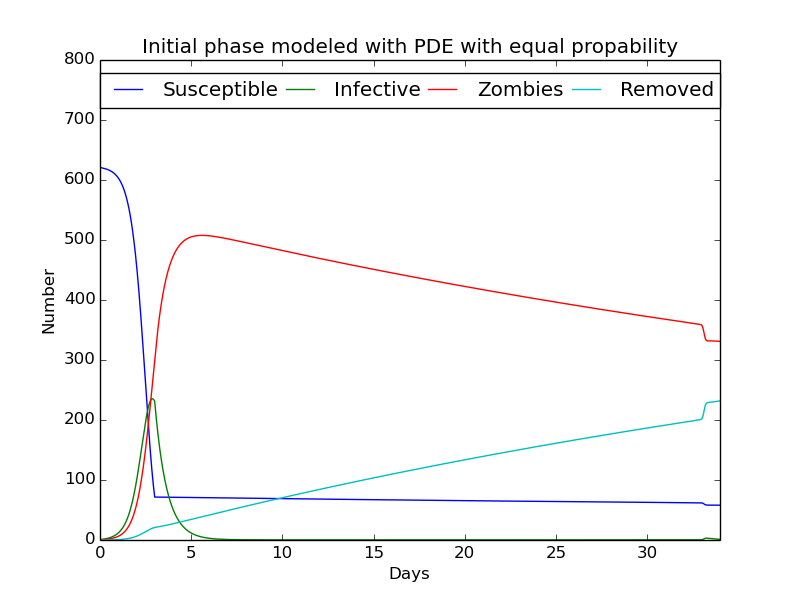
\includegraphics[width=0.8\linewidth]{2_fig/2D_zombie_three_phases_number.png}}
  \caption{
  \label{fig:zombie_three_number} The Eq.(\ref{eq:SIZR_disc2}) modeled with uniformed distributed groups. Initial values $S_0 = 621$, $I_0 = 0$, $Z_0 = 0$ and  $R_0 = 0$ with parameters from (\ref{table:param_val}).
  }
\end{figure}
%\clearpage % flush figures fig:zombie_three_number




\vspace{3mm}




\vspace{3mm}


The initial values for the four groups are set to $S_0=621$, $I_0=0$, $Z_0=1$ and $R_0= 0$ in all simulations. The values in Tab.(\ref{table:compare_phases_zombie}) are measured at the final time for each phase. The \emph{Initial phase} lasts for three days and the values are measured at $time=3$. The \emph{Hysterical phase} is a continuous phase, and will not stop until an eventual eradication. The values are therefore given before the \emph{Counter attack} at $time=33$. The \emph{Counter attack} lasts for some hours, and is measured at $time=34$, which is a day after the attack. The value of $\Delta t$ is set to 1E-3. 

\label{table:compare_phases_zombie}

\begin{quote}
\begin{tabular}{cccc}
\hline
\multicolumn{1}{c}{  } & \multicolumn{1}{c}{ ODE system } & \multicolumn{1}{c}{ PDE uniform dist } & \multicolumn{1}{c}{ PDE gauss center } \\
\hline
Initial phase    & ----------- & ------------------- & ------------------- \\
\hline
Susceptible      & 71.3        & 71.3                & 81.12               \\
Infected         & 230.8       & 230.8               & 210.94              \\
Zombie           & 298.9       & 298.9               & 310.11              \\
Removed          & 21.0        & 21.0                & 20.60               \\
\hline
Hysterical phase & ----------- & ------------------- & ------------------- \\
\hline
Susceptible      & 61.6        & 61.6                & 70.55               \\
Infected         & 0.3         & 0.3                 & 0.34                \\
Zombie           & 358.6       & 355.6               & 334.33              \\
Removed          & 201.5       & 201.5               & 217.56              \\
\hline
Counter attack   & ----------- & ------------------- & ------------------- \\
\hline
Susceptible      & 57.8        & 57.8                & 66.50               \\
Infected         & 1.2         & 1.2                 & 1.23                \\
Zombie           & 331.8       & 331.8               & 305.86              \\
Removed          & 231.3       & 231.3               & 249.19              \\
\hline
\end{tabular}
\end{quote}

\noindent
These results shows that the PDE system gives the same results as the ODE system.

% #
% #
% #
% #


\subsection{The position of the \emph{Infected} group}
In the previous section, \emph{English boarding school}, the location of the \emph{Infected} group was proven to have a major influence on the result. However here the \emph{Susceptible} group was uniformly distributed over the schoolyard. The number in each group, based on the study of \emph{Walking Dead}, was seen in three different locations in the TV series. By only studying the TV series, it is hard to decide the geographical distance between these three locations. Therefore they have been placed with a certain distance from each other. The following simulations are done on a grid with size(40 x 40) with the following positions for the towns: Small town(6,6) with size 21, middle town(12,25) with size 200 and large town(25,12) with size 400. Since these values were based on the humans and zombies seen in the series, these can be scaled up by 1000 to correspond a realistic population. A large town can be seen as an area with a population of 400 000. The length can be measured in kilometres. Then the distance between the middle and large town will be 18.38 km. Compared to the distance between Oslo and Bærum(Sandvika) which is 15 km, the simulation can be seen as a rough estimate of the area around Oslo, if the fjord is frozen and the mobility for the area is similar.


\vspace{3mm}




\vspace{3mm}


The diffusion term describes the diffusion for each group. This can be seen as the speed towards equilibrium for each group. If the diffusion constant is large, the flow towards equilibrium will go faster. The values have been set as follows. 
\begin{itemize}
\item $D_s=1$, The \emph{Susceptible} has a basic moving speed. The other groups are based on the speed of a healthy human.

\item $D_i=0.5$, The \emph{Infected} are often injured caused by recent fights. This affects their mobility.

\item $D_z=0.9$, The average moving speed for a zombie. There are zombies with the mobility of a human, but there are also zombies that drag themselves forward with only one arm. This results in a major difference in speed and therefore a lower average speed for the zombies.

\item $D_r=0$, The removed are here seen as dead, therefore there is no mobility.
\end{itemize}

\noindent


\vspace{3mm}




\vspace{3mm}


The parameters from Tab.(\ref{table:param_val}) will be used here, and the three phases will be modeled as shown for the uniformed distributed PDE system. The values will be used for three different simulations with the similar initial value for the different groups. The position of initial values can be seen in Fig.(\ref{fig:initial_value_susceptible}) and are based on the data given for each town above. The difference in the three simulations will be the position of the zombie at initial time. The zombie will be placed in center of the small, middle and large town.


\begin{figure}[ht]
  \centerline{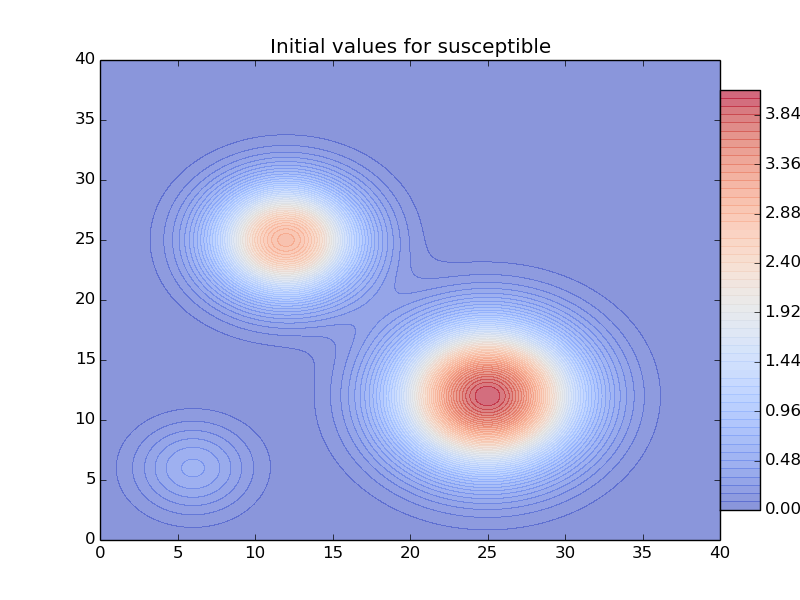
\includegraphics[width=0.8\linewidth]{2_fig/initial_value_susceptible.png}}
  \caption{
  \label{fig:initial_value_susceptible} The initial value for the \emph{Susceptible} group for three simulations. Small group(6,6) with volume 21, middle group(12,25) with volume 200 and large group(25,12) with volume 400. All three groups are build up with a Gaussian function.
  }
\end{figure}
%\clearpage % flush figures fig:initial_value_susceptible




\vspace{3mm}




\vspace{3mm}


Fig.(\ref{fig:large_town}) shows the simulation where the zombie is placed in the large town. The simulations of the small and middle town can be seen in the Appendix. The four subplots are from the different phases that arise during a zombie attack. The different groups have the same color as introduced in Fig.(\ref{fig:zombie_three_number}). It is difficult to separate the three groups \emph{Infected}, \emph{Zombie} and \emph{Removed}, since they all have a low value at initial time. The development of the amount can easier be seen in the Fig.(\ref{fig:compare_towns}), which also shows the results from the small and middle town. Since the amount of \emph{Susceptible} is quite low in the small town where the zombie arises, the disease is not able to infect too many before the society has moved to the next phase, assuming that the broadcasting about the disease works okay for the first days. This results in an eradication of the disease in about a month. The table(\ref{table:compare_phases_zombie}) shows that the number of zombies decreases towards zero after a month. 


\begin{figure}[ht]
  \centerline{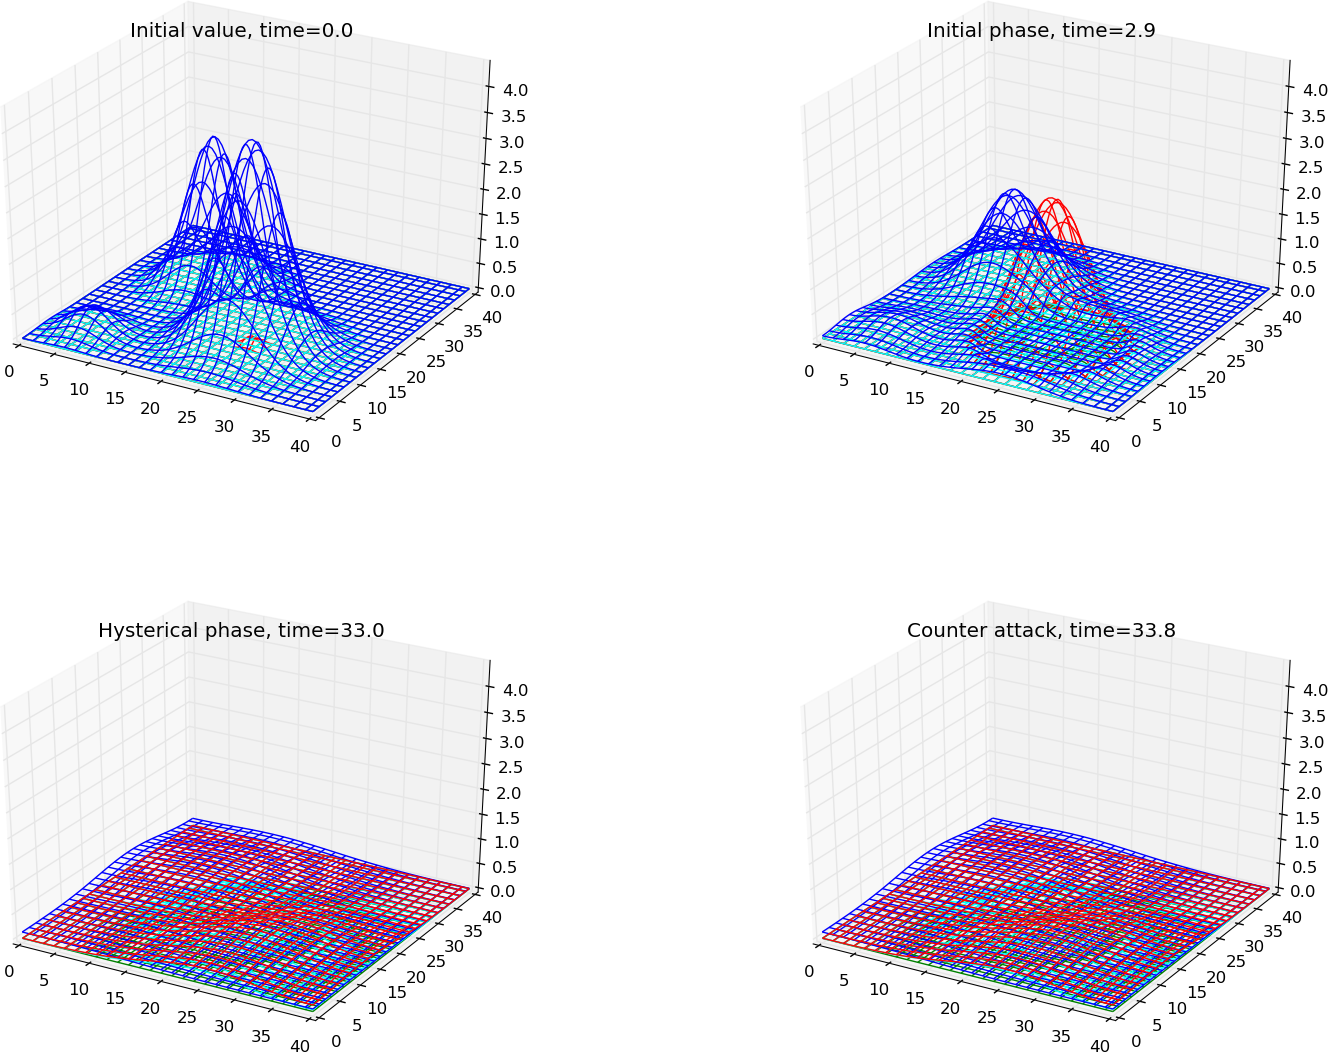
\includegraphics[width=0.8\linewidth]{2_fig/2D_zombie_three_phases_zombie_large_town_2_sub.png}}
  \caption{
  \label{fig:large_town} \emph{Walking Dead} simulated with the zombie at initial time in the large town. Subplots shown at each phase.
  }
\end{figure}
%\clearpage % flush figures fig:large_town




\vspace{3mm}




\vspace{3mm}


By placing the zombie in the middle town, the amount in the \emph{Zombie} group increases to a higher level. The amount can be seen as subplot II in Fig.(\ref{fig:compare_towns}). The damages are higher, and after a month the total population of \emph{Susceptible} is reduced to 427. The last calculation done for the large town in Fig.(\ref{fig:large_town}) shows major damages. Here the amount in the \emph{Zombie} group increases above the number of \emph{Susceptible}. The \emph{Infected} group also increases to above 100 after a couple of days in the initial phase. This can be explained by the high number of meetings between susceptible and zombies. By studying the subplot II in Fig.(\ref{fig:large_town}), the zombies are grouped in the large town, while the middle and small town mostly consist of \emph{Susceptible}. By counting the loss of \emph{Susceptible} during the first phase, the Tab.(\ref{table:compare_towns}) shows that this amount corresponds with the size of the towns where the zombie was placed, given by the number 17,188 and 362 in the small,middle and large group. The percent is highest in the middle town with 94 percent. The percent in the large and small group are 90 and 81.  The simulation in the middle town has the highest percent because the \emph{Susceptible} group in the large town also gets infected. These towns are coupled together, and the epidemic disease is able to spread. The small town, which can be seen as Nesodden(a peninsula outside Oslo), has the lowest percent. The reason is that the disease is not able to spread to the other towns, and therefore is causes less damage.  


\begin{figure}[ht]
  \centerline{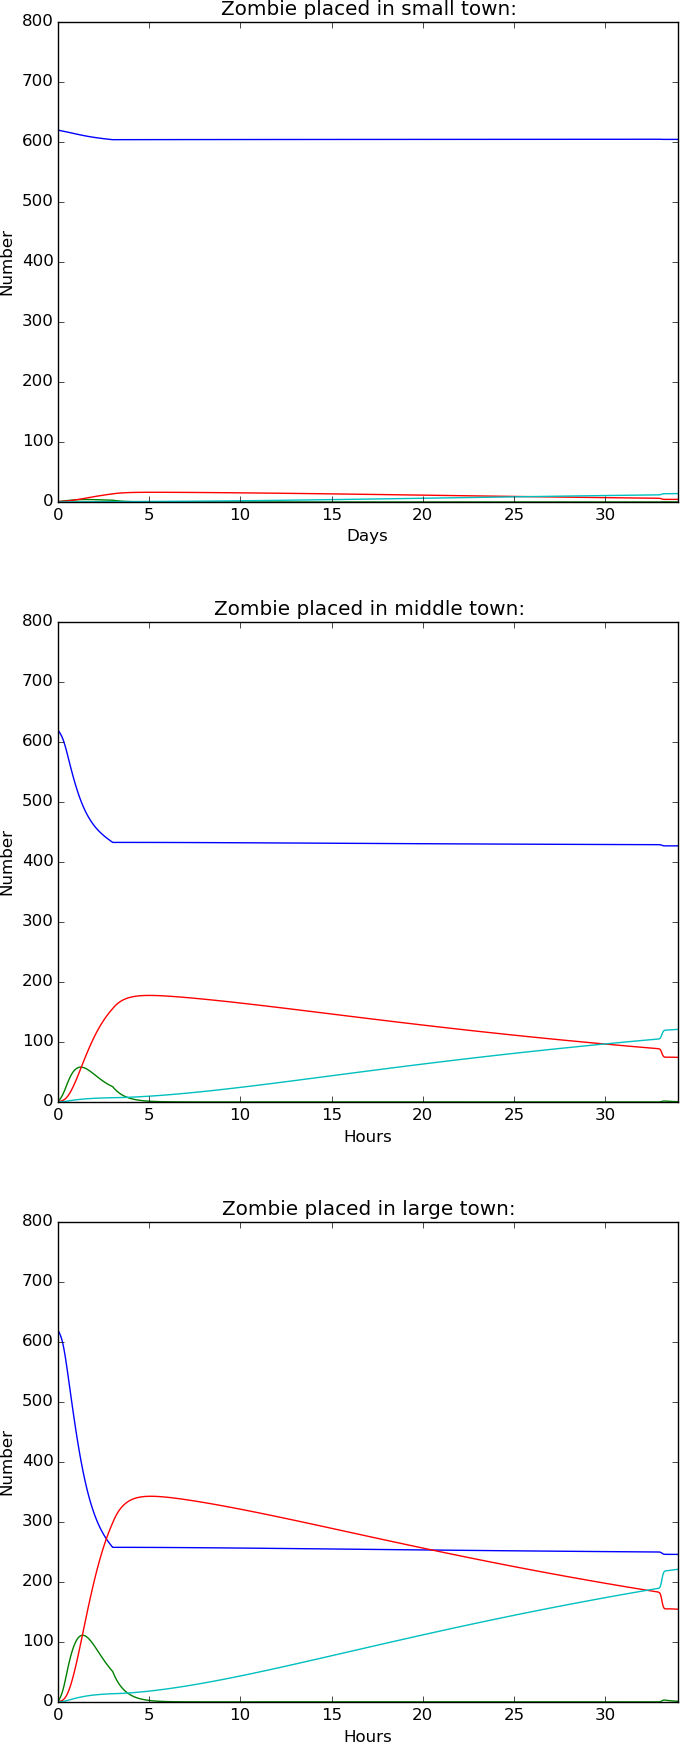
\includegraphics[width=0.6\linewidth]{2_fig/2D_compare_towns.png}}
  \caption{
  \label{fig:compare_towns} The values for each group counted during 34 days in \emph{Walking Dead}. Initial phase from day 0 to day 3, Hysterical phase from day 3 to day 33 and Counter attack from day 33 to day 34.
  }
\end{figure}
%\clearpage % flush figures fig:compare_towns




\vspace{3mm}




\vspace{3mm}


The results from the uniformed distributed simulation is still much higher for the \emph{Zombie} group the in these three simulations. This shows that using the parameters from the ODE system in a geographical area makes little sense. A realistic assumption is that a zombie is restricted to a given area, and therefore the parameters will not be equal for all. The chance of getting infected is much higher if a person from the  \emph{Susceptible} group is close to an infected. There is also a greater chance of getting infected if the \emph{Susceptible} group has a high density. 

% FIGURE:[2_fig/2D_zombie_three_phases_zombie_small_town_2_number.png, height=600 width=800 frac=0.8]

% FIGURE:[plots/2D_zombie_three_phases_zombie_middle_town_2_number.png, height=600 width=800 frac=0.8]

% FIGURE:[plots/2D_zombie_three_phases_zombie_large_town_2_number.png, height=600 width=800 frac=0.8]





\label{table:compare_towns}

\begin{quote}
\begin{tabular}{cccc}
\hline
\multicolumn{1}{c}{  } & \multicolumn{1}{c}{ Small town } & \multicolumn{1}{c}{ Middle town } & \multicolumn{1}{c}{ Large } \\
\hline
Initial phase    & ----------- & ------------------- & ------------------- \\
\hline
Susceptible      & 603.74      & 433.22              & 259.20              \\
Infected         & 2.96        & 25.51               & 50.94               \\
Zombie           & 13.79       & 155.27              & 297.24              \\
Removed          & 0.66        & 7.16                & 13.78               \\
\hline
Hysterical phase & ----------- & ------------------- & ------------------- \\
\hline
Susceptible      & 604.42      & 429.35              & 251.14              \\
Infected         & 0.03        & 0.18                & 0.35                \\
Zombie           & 6.25        & 87.31               & 178.45              \\
Removed          & 12.14       & 106.00              & 192.90              \\
\hline
Counter attack   & ----------- & ------------------- & ------------------- \\
\hline
Susceptible      & 604.21      & 427.45              & 247.33              \\
Infected         & 0.08        & 0.59                & 1.17                \\
Zombie           & 4.49        & 73.70               & 151.44              \\
Removed          & 14.11       & 121.16              & 222.96              \\
\hline
\end{tabular}
\end{quote}

\noindent
\subsection{Free areas for the \emph{Susceptible} group}
To model a realistic zombie attack, humans ability to think logically is crucial in the fight. The mobility was presented as a factor in the previous section. Another important skill that the \emph{Susceptible} group holds, is the ability to decide the safety of an area. In the TV series \emph{Walking Dead}, the humans build barricades to keep the zombies outside. This gives the \emph{Susceptible} group free areas where they can stay. This idea can be transfered to the PDE system by rewriting the Eq.(\ref{eq:seland_model_PDE}) with spatial dependent diffusion terms. The diffusion constant $D_u$ is now replaced with a diffusion function $\gamma_u(x)$ for $u= S,I,Z,R$, which is spatial discretized. Since a diffusion equation always goes towards equilibrium, this rewriting will only slow down/stop the selected group to diffuse into an area. In this case it will stop the \emph{Zombie} group from diffusing into the buildings. 
\begin{equation} \label{eq:seland_model_diff}
    \begin{aligned} 
    \frac{\partial S}{\partial t} =& \Sigma -(\beta+\mu \omega(t))SZ - \delta_SS +\nabla(\gamma_S(x) \nabla S) \\
    \frac{\partial I}{\partial t} =& (\beta+\mu \omega(t))SZ - \varrho I - D_i\delta_II+\nabla(\gamma_I(x) \nabla I)\\
    \frac{\partial Z}{\partial t} =& \varrho I- (\alpha+\omega(t))SZ + \zeta R+\nabla(\gamma_Z(x) \nabla Z)\\
    \frac{\partial R}{\partial t} =& \delta_SS +\delta_II -\zeta R + (\alpha+\omega(t))SZ+\nabla(\gamma_R(x) \nabla R) 
    \end{aligned}
\end{equation}
The diffusion term is the difference between this system and Eq.(\ref{eq:seland_model_PDE}). The discretization can be shown for for a general $\gamma$. This will be similar for all groups. A centered difference is used in space.
\begin{equation} \label{eq:gamma}
    \begin{aligned}
    &=\nabla(\gamma(x) \nabla S) \\
    &=(\gamma(x) S_x)_x+(\gamma(x) S_y)_y \\
    &= \left(\gamma(x) \frac{S^{n}_{i+1/2,j}-S^{n}_{i-1/2,j}}{\Delta x}\right)_x+\left(\gamma(x) \frac{S^{n}_{i,j+1/2}-S^{n}_{i,j-1/2}}{\Delta y}\right)_y \\
    &= \left(\frac{\gamma(x_{i+1/2,j})(S^{n}_{i+1,j}-S^{n}_{i,j})-\gamma(x_{i-1/2,j})(S^{n}_{i,j}-S^{n}_{i-1,j})}{\Delta x^2}\right) \\
    &+ \left(\frac{\gamma(x_{i,j+1/2})(S^{n}_{i,j+1}-S^{n}_{i,j})-\gamma(x_{i,j-1/2})(S^{n}_{i,j}-S^{n}_{i,j-})}{\Delta y^2}\right)
    \end{aligned}
\end{equation}
Since the calculations are based on spatial points, the values inside the function of $\gamma$ need to be adjusted. This can be done by the use of an arithmetic mean, which can be seen in Eq.(\ref{eq:arith_mean}). The notation $q_{i+1/2}$ is a simplification of the function $q(x_{i+1/2})$ with $x_{i+1/2} = x_i + 1/2 \Delta x$
\begin{equation} \label{eq:arith_mean}
q_{i+1/2} \approx \frac{1}{2}(q_i +q_{i+1})
\end{equation}
This arithmetic mean can be inserted for all $\gamma$'s in the system. The system can be expressed:
\begin{equation} \label{eq:SIZR_disc3}
	\begin{aligned}
    S^{n+1}_{i,j}   &= S^n_{i,j} + \Delta t \Bigl( \Sigma - (\beta+\mu \omega(t))S^{n}_{i,j}Z^{n}_{i,j}- \delta_S S^{n}_{i,j} \\
                    &+ \frac{1}{2\Delta x^2}\left(\gamma_S(x_{i-1,j})(S^{n}_{i-1,j}-S^{n}_{i,j})+\gamma_S(x_{i,j})(S^{n}_{i-1,j}-2S^{n}_{i,j}+S^{n}_{i+1,j})+\gamma_S(x_{i+1,j})(-S^{n}_{i,j}+S^{n}_{i+1,j})\right) \\
                    &+ \frac{1}{2\Delta y^2}\left(\gamma_S(x_{i,j-1})(S^{n}_{i,j-1}-S^{n}_{i,j})+\gamma_S(x_{i,j})(S^{n}_{i,j-1}-2S^{n}_{i,j}+S^{n}_{i,j+1})+\gamma_S(x_{i,j+1})(-S^{n}_{i,j}+S^{n}_{i,j+1})\right)\Bigr)\\
    I^{n+1}_{i,j}   &= I^n_{i,j} + \Delta t \Bigl((\beta+\mu \omega(t))S^{n}_{i,j}Z^{n}_{i,j}-\varrho I^{n}_{i,j}- \delta_I I^{n}_{i,j} \\
                    &+ \frac{1}{2\Delta x^2}\left(\gamma_I(x_{i-1,j})(I^{n}_{i-1,j}-I^{n}_{i,j})+\gamma_I(x_{i,j})(I^{n}_{i-1,j}-2I^{n}_{i,j}+I^{n}_{i+1,j})+\gamma_I(x_{i+1,j})(-I^{n}_{i,j}+I^{n}_{i+1,j})\right) \\
                    &+ \frac{1}{2\Delta y^2}\left(\gamma_I(x_{i,j-1})(I^{n}_{i,j-1}-I^{n}_{i,j})+\gamma_I(x_{i,j})(I^{n}_{i,j-1}-2I^{n}_{i,j}+I^{n}_{i,j+1})+\gamma_I(x_{i,j+1})(-I^{n}_{i,j}+I^{n}_{i,j+1})\right)\Bigr)\\
    Z^{n+1}_{i,j}   &= Z^n_{i,j} +\Delta t \Bigl( \varrho I^{n}_{i,j}-(\alpha+\omega(t))S^{n}_{i,j}Z^{n}_{i,j}+ \zeta R^{n}_{i,j} \\
                    &+ \frac{1}{2\Delta x^2}\left(\gamma_Z(x_{i-1,j})(Z^{n}_{i-1,j}-Z^{n}_{i,j})+\gamma_Z(x_{i,j})(Z^{n}_{i-1,j}-2Z^{n}_{i,j}+Z^{n}_{i+1,j})+\gamma_Z(x_{i+1,j})(-Z^{n}_{i,j}+Z^{n}_{i+1,j})\right) \\
                    &+ \frac{1}{2\Delta y^2}\left(\gamma_Z(x_{i,j-1})(Z^{n}_{i,j-1}-Z^{n}_{i,j})+\gamma_Z(x_{i,j})(Z^{n}_{i,j-1}-2Z^{n}_{i,j}+Z^{n}_{i,j+1})+\gamma_Z(x_{i,j+1})(-Z^{n}_{i,j}+Z^{n}_{i,j+1})\right)\Bigr)\\
    R^{n+1}_{i,j}   &= R^n_{i,j} +\Delta t \left(\delta_S S^{n}_{i,j}+\delta_I I^{n}_{i,j}-\zeta R^{n}_{i,j}+(\alpha+\omega(t))S^{n}_{i,j}Z^{n}_{i,j}\right)
	\end{aligned}
\end{equation}
The diffusion term for the \emph{Removed} group is taken away, since dead people are not able to move. This system looks quite messy, but it is straight forward to calculate. All values on the right side are known values and the system is easy to solve. Now every point will be controlled by the diffusion constants given in $\gamma(x)$. This makes it easier to control the flow in each group. With a high diffusion constant, the diffusion will spread fast. When the diffusion constant goes towards zero, the flow will decrease towards zero flow. This will result in a set of ODE systems modeled for each point.

\subsection{Ten minutes at Frederikkeplassen}
Frederikkeplassen at the University of Oslo is a possible area for an upcoming zombie attack. This simulation will try to model a ten minute sequence with the diffusion parameter added in this section. Since students often learn and interact fast, they will only use three minutes before they realize the danger and transitions into the \emph{Hysterical phase}. A map of Frederikkeplassen is used to define the safe and critical areas. The buildings are set as areas where only the \emph{Susceptible} are allowed to move. This is done by setting the diffusion constant to zero for the \emph{Zombie} and \emph{Infected} groups. Since the buildings are safe spots for the \emph{Susceptible}, an idea would be to express this in the diffusion term by forcing the \emph{Susceptible} for other areas into the buildings. This is more difficult, since the concentrations in each group wants to diffuse towards equilibrium. A way to delay this process is by setting the diffusion constant to be low in the buildings and high outside. This will result in a fast diffusion in the open areas and a slow diffusion inside the buildings. 


\begin{figure}[ht]
  \centerline{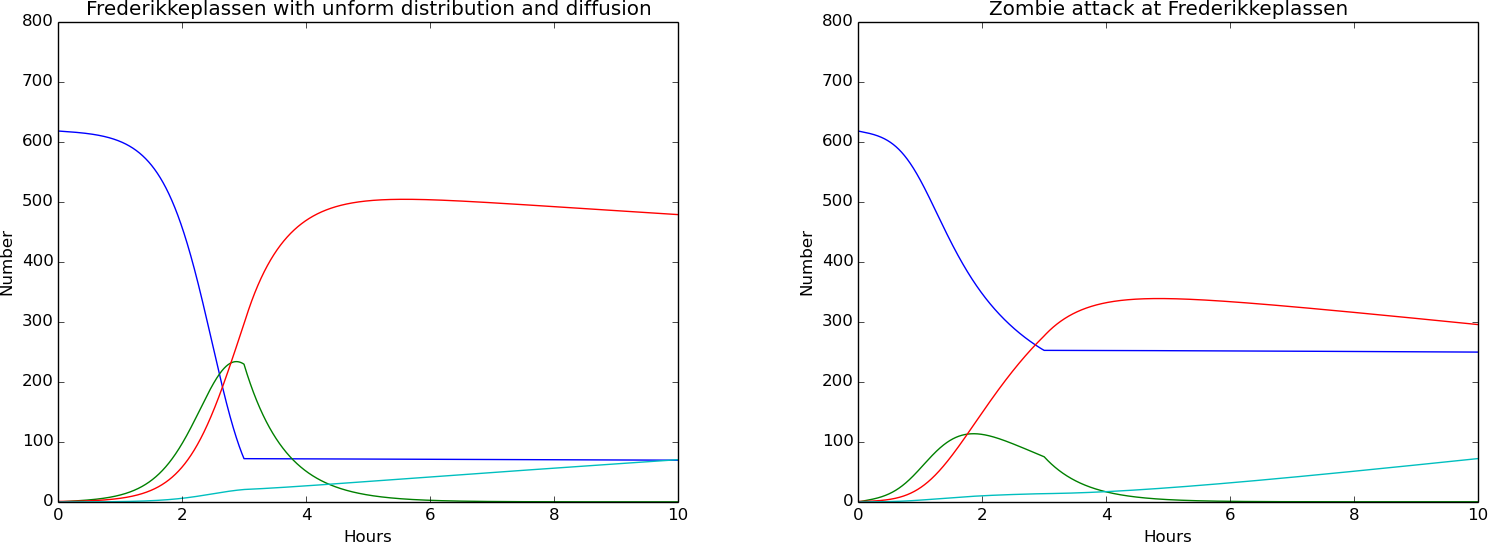
\includegraphics[width=0.8\linewidth]{2_fig/2D_compare_Frederikke.png}}
  \caption{
  \label{fig:frederikke_numbers} The amount in each group for two simulations of Frederikkeplassen modeled same parameters for 10 minutes/hours. a)Plot with uniformed distributed groups and same diffusion constants for all groups. b)Plot based on figure(\ref{fig:frederikke_free_area}) with different initial values for each group.
  }
\end{figure}
%\clearpage % flush figures fig:frederikke_numbers




\vspace{3mm}




\vspace{3mm}


Two simulations have been done at Frederikkeplassen. The amount in each group can be seen in Fig.(\ref{fig:frederikke_numbers}). The first simulation has a solution based on the ODE system, with uniformed distributed groups, equal diffusion constants and no free areas for the \emph{Susceptible}. The second simulation is modeled with three groups of \emph{Susceptible}, as in the previous section. The small group with 21 students is placed at point(4,4), the middle group with 200 students is placed at point(15,8) and the large group with 400 students is placed at point(8,13). The zombie is placed at point(8,10). The $\gamma(x)$ is set to zero in the buildings for the \emph{Zombie} and \emph{Infected} group, and one in the rest of the area. For the \emph{Susceptible} group, $\gamma(x)$ is set to 0.1 in the buildings, which causes slow diffusion. In the outside areas, $\gamma(x)$ is set to 5 for the \emph{Susceptible}. The desired result is to push them into the buildings, but this will only happen if there is a lower concentration inside the buildings. Therefore this will not reflect a realistic flow of a \emph{Susceptible} population. This simulation can be seen in Fig.(\ref{fig:frederikke_free_area})  


\begin{figure}[ht]
  \centerline{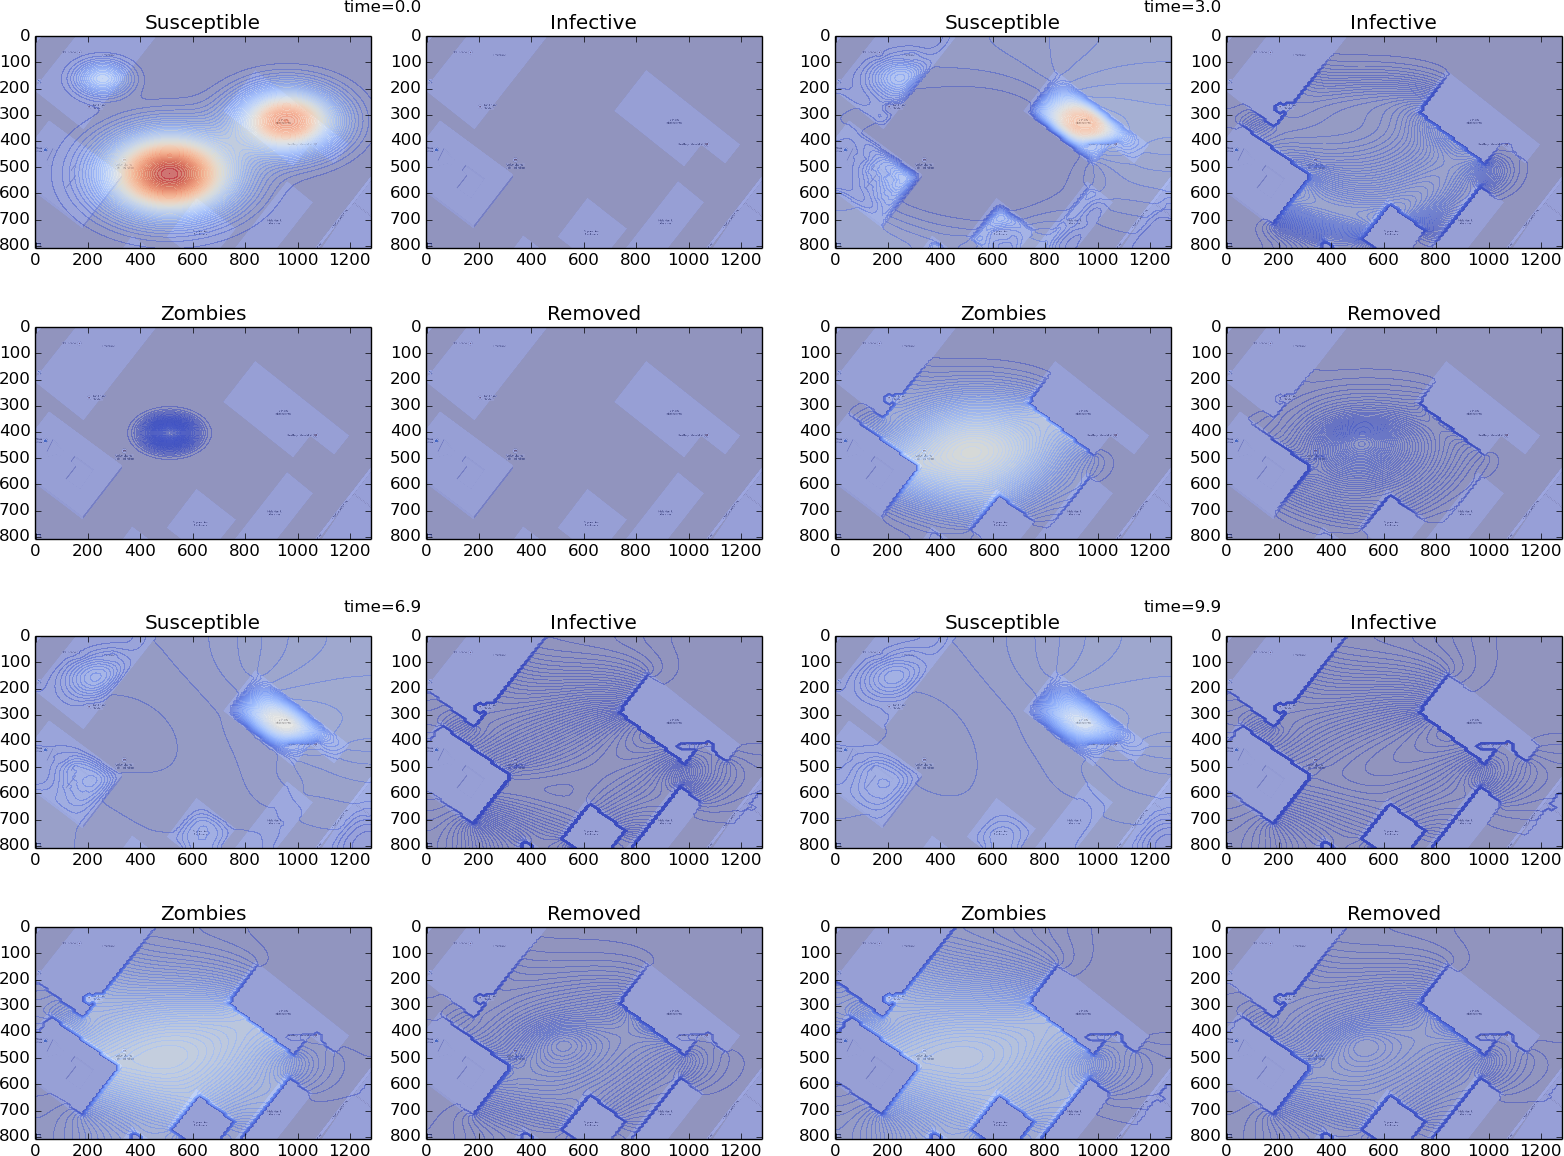
\includegraphics[width=0.8\linewidth]{2_fig/2D_Frederikke_contourf_sub.png}}
  \caption{
  \label{fig:frederikke_free_area} Frederikkeplassen modeled with free areas for the \emph{Susceptible} group. The diffusion function $\gamma(x)$ is set to zero for the \emph{Zombie} and \emph{Infected} group in the buildings. The zombie at initial time is placed in the center of Frederikkeplassen
  }
\end{figure}
%\clearpage % flush figures fig:frederikke_free_area




\vspace{3mm}




\vspace{3mm}


The results in Tab.(\ref{table:frederikke_table}) shows that the three first minutes are crucial. The number after three minutes shows that only 72 humans survived the attack in the uniformed solution, compared to 252 in the free areas. The number in the \emph{Zombie} group is quite similar in \emph{Uniformed distribution} and \emph{Free areas} measured at $t=3$. However at $t=7$ the difference is major. This can be explained by looking at Fig.(\ref{fig:frederikke_free_area}) and the building with the middle group placed inside. When the zombie starts attacking at $t=0$, the large group is exposed. This group is placed close to the zombie and the position is in an open area. The zombie can attack right away and the number in the \emph{Infected} and \emph{Zombie} groups increases fast. In the two first minutes, a major part of the large group is infected and the \emph{Zombie} group starts to spread. After 2-3 minutes, the group has reached the buildings with the middle group. Here the diffusion is set to 0, and the spread of zombies stop. Since the diffusion variable for the \emph{Susceptible} is quite low inside the buildings, it takes time before the group diffuses. Maybe the right diffusion value along the buildings would be 0, to avoid any leakage. This would again cause problem for the diffusion of \emph{Susceptible} into the buildings. It is also reasonable to think that the \emph{Susceptible} group needs to diffuse after a certain time. The lack of supplies would force them out.

\label{table:frederikke_table}

\begin{quote}
\begin{tabular}{ccc}
\hline
\multicolumn{1}{c}{  } & \multicolumn{1}{c}{ Uniform distribution } & \multicolumn{1}{c}{ Free areas } \\
\hline
3 Minutes   & --------------------------- & --------------- \\
\hline
Susceptible & 72.23                       & 252.72          \\
Infected    & 229.65                      & 75.69           \\
Zombie      & 296.67                      & 276.55          \\
Removed     & 20.84                       & 13.94           \\
\hline
7 Minutes   & --------------------------- & --------------- \\
\hline
Susceptible & 70.78                       & 251.35          \\
Infected    & 0.83                        & 0.51            \\
Zombie      & 498.72                      & 325.54          \\
Removed     & 49.12                       & 41.26           \\
\hline
10 Minutes  & --------------------------- & --------------- \\
\hline
Susceptible & 69.69                       & 249.84          \\
Infected    & 0.25                        & 0.38            \\
Zombie      & 479.00                      & 295.71          \\
Removed     & 70.55                       & 72.36           \\
\hline
\end{tabular}
\end{quote}

\noindent

\section{Discussion}
This chapter expand the study of the disease, by adding the opportunity to analyse the disease for a spatial area. The travelling wave is essential for a disease to spread in an area. If the reproduction rate seen in Eq.(\ref{eq:reproduction_rate_PDF}) was below 1, the travelling wave would decrease towars zero and the disease would dissapear. By varying $\lambda$, one could see that a low value would cause a total eradication of the \emph{Susceptible}. By setting $\lambda>=1$, the damage from the epidemic wave would be close to zero and the disease would die out.


\vspace{3mm}




\vspace{3mm}


The results from the English boarding school shows that the position of the infected student has a major impact on the result. A uniform distribution was first calculated and compared with the ODE simulation in the previous chapter. This gave the same result. By varying the position of the infected student, the result was affected. When simulating the disease for a long time, the number of \emph{Infected} students seems to be similar. Therefore the parameter values in the system will not be enough to say anything about the concentrations measured in time for each group. The position will also affect the result. 


\vspace{3mm}




\vspace{3mm}


The section \emph{Zombiefication} verified the uniform distribued PDF solution with the ODE solution from the previous chapter. These were expected to be similar. The English boarding school studied the result of varying the position of the infected with a uniform distributed group of \emph{Susceptible}. This section tried to expand this idea byspread the group of \emph{Susceptible} into three groups. The position of the zombie was placed in center of all three groups. The amount of \emph{Infected} in these three simulations was proportional to the size of the group where the zombie was placed. The position of the infected student was shown to have an impact on the spread of the disease. This section shows that the \emph{Susceptible} group also affects the result.


\vspace{3mm}




\vspace{3mm}


The last part \emph{Ten minutes at Frederikke} tries to implement human behavior by giving the \emph{Susceptible} group the ability to keep zombies outside the buildings. This was crucial in \emph{Walking Dead} to prevent meetings between zombies and humans. One can see from the results that this gives the \emph{Susceptible} group a greater chance of surviving. The concentrations for each group will go towards equilibrium. Therefore this simulation will differ from human behavior. The next chapter will use random walks to simulate this zombie outburst. This will build on \emph{Ten minutes ad Frederikke}, and introduce different conditions based on the phase the zombies and humans are in. 




\clearemptydoublepage
\markboth{Bibliography}{Bibliography}
\thispagestyle{empty}

\bibliographystyle{plain}
\bibliography{../bibliography/papers}


% ------------------- end of main content ---------------


\clearemptydoublepage
\markboth{Index}{Index}
\thispagestyle{empty}
\printindex

\end{document}

